\pdfobjcompresslevel 0
\documentclass[11pt, twoside, a4paper]{memoir}

%====================================================
%					PREAMBLE
%====================================================

%Page de garde
\usepackage[a4paper]{meta-donnees}

%Font encoding
\usepackage[utf8]{inputenc}
\usepackage[T1]{fontenc}
\usepackage{lmodern}

% Chapter styles
%\chapterstyle{madsen}

% Sans serif headers - indented
%\renewcommand{\parttitlefont}{\HUGE\bfseries\sffamily\scshape}
%\renewcommand{\chaptitlefont}{\HUGE\bfseries\sffamily\scshape}
%\setsecheadstyle{\LARGE\sffamily\scshape\raggedright\bfseries}
%\setsubsecheadstyle{\large\sffamily\bfseries\raggedright}
%\setsubsubsecheadstyle{\sffamily\bfseries\itshape\raggedright}
%\setparaheadstyle{\sffamily\itshape\raggedright}

% table of contents font customization
%\renewcommand{\cftchapterfont}{\sffamily\scshape{}\bfseries{}\large}
%\renewcommand{\cftsectionfont}{\sffamily\scshape{}}
%\renewcommand{\cftsubsectionfont}{\sffamily\scriptsize}
%\renewcommand{\cftsubsubsectionfont}{\scriptsize}

% Header and footer style
\makepagestyle{ruled}
\makeevenhead{ruled}{\normalsize\leftmark}{}{\normalsize}
\makeoddhead{ruled}{\normalsize}{}{\normalsize\rightmark}
\makeevenfoot{ruled}{\normalsize\thepage}{}{\normalsize}
\makeoddfoot{ruled}{\normalsize}{}{\normalsize\thepage}
\makeheadrule{ruled}{\textwidth}{0.1pt}
\pagestyle{ruled} 

%Lettrine
\usepackage{lettrine}
\newcommand{\Lettrine}[2]{\lettrine[lines=4]{\textcolor{Blue}{#1}}{#2}}

%Biblio
\usepackage[backend=biber, 
			style=alphabetic, 
			isbn=false,
			doi=false,
			url=false,
			backref=false,
			giveninits=false, 
			maxcitenames=2,
			maxbibnames=100]{biblatex}
\usepackage{csquotes}

\addbibresource{./bib/thesis_manteaux.bib}

%Units
\usepackage[squaren,Gray]{SIunits}

%Images
%\ifpdf \usepackage[pdftex]{graphicx} \pdfcompresslevel=9
%\else \usepackage[dvips]{graphicx} \fi

%Alignement
\usepackage[export]{adjustbox} % add valign=<t,m,b> option to \includegraphics

%Maths
\usepackage{amsmath}
\usepackage{amssymb}

%Color and highlighting
\usepackage{transparent}
\usepackage{soul} % highlighting with word wrap
\newcommand{\highlight}[2]{\colorlet{hlcolor}{#1}\sethlcolor{hlcolor}\hl{#2}} % work around soul/xcolor conflict
\usepackage[usenames,dvipsnames]{xcolor}

%Math commands
\renewcommand{\vec}[1]{\mathbf{#1}}
\newcommand{\vp}{\vec{p}}
\newcommand{\vq}{\vec{q}}
\newcommand{\vx}{\vec{x}}
\newcommand{\vf}{\vec{f}}
\renewcommand{\H}{\mathcal{H}}

%Algorithms
\usepackage{algorithm}
\usepackage{algpseudocode}
\algnewcommand{\LineComment}[1]{\State \(\triangleright\) #1}

%Improvement
\usepackage[activate={true,nocompatibility},
			final,tracking=true,
			kerning=true,
			spacing=true,
			factor=1000,
			stretch=10,
			shrink=10]{microtype}
\microtypecontext{spacing=nonfrench}

%Subfigure
\usepackage{subcaption}

%Highlighting command
\newcommand{\TODO}[1]{\highlight{Orange!40}{TODO: #1}}

%Table of contents settings
\settocdepth{subsubsection}
\setsecnumdepth{subsubsection}

\usepackage{epstopdf}

%Orphans
\widowpenalty=10000
\clubpenalty=10000

%Hyperref
\usepackage[colorlinks=true,
            linkcolor=blue,
            urlcolor=blue,
            citecolor=blue]{hyperref}

%Space after each para break
%\setlength{\parskip}{\baselineskip}
\setlength{\parskip}{1pt}

%Indent new paragraphs by 0pt (so no indent)
%\setlength{\parindent}{0pt}%


%====================================================
%				    GLOSSARY	
%====================================================
\usepackage[acronym, nonumberlist, nopostdot, section]{glossaries}
\usepackage{glossary-longbooktabs} 

\setglossarystyle{long-booktabs}
\renewcommand*{\glossaryname}{Notations}
\renewcommand*{\entryname}{Symbol}
\renewcommand*{\descriptionname}{Description}

\makeglossaries

%Main glossary

%Acronym glossary
\newacronym{arps}{ARPS}{Adaptively Restrained Particles Simulations}
\newacronym{bcc}{BCC}{Body-centered cubic}
\newacronym{mls}{MLS}{Moving Least Squares}
\newacronym{sph}{SPH}{Smoothed-Particle Hydrodynamics}

%Symbol glossary
\newglossaryentry{Omega}{name={\ensuremath{\Omega}},symbol={\ensuremath{\Omega}},description={Simulation domain}}
\newglossaryentry{Divergence}{name={\ensuremath{\nabla \cdot}},symbol={\ensuremath{\nabla \cdot}},description={Divergence operator}}
\newglossaryentry{Gradient}{name={\ensuremath{\nabla}},symbol={\ensuremath{\nabla}},description={Gradient operator}}
\newglossaryentry{Laplacian}{name={\ensuremath{\Delta}},symbol={\ensuremath{\Delta}},description={Laplacian operator}}

%====================================================
%					DOCUMENT
%====================================================

\begin{document}

\title{Simulation and control of physical phenomena}
\author{Pierre-Luc Manteaux}
%\date{\today}
%\maketitle

% les lignes en bas sont à insérer obligatoirement après \begin{document}

%%%%%%%%%%%%%%%%%%%%%%%%%%%%%%%%%%%%%%%%%%%%%%%%%%%%%%
%%             Commandes Meta-données               %%
%%   à renseigner par les auteurs pour générer      %%
%%     la couverture modèle Univ. Grenoble          %%
%%%%%%%%%%%%%%%%%%%%%%%%%%%%%%%%%%%%%%%%%%%%%%%%%%%%%%
%%      Fichier encodé au format ISO-8859-16        %%

%\Sethpageshift{???mm}   %%optionnel : à décommenter si besoin pour ajout d'espace afin de center la couvérture horizontalement (valeur par défaut est -5.5mm)
%\Setvpageshift{???mm}   %%optionnel : à décommenter si besoin pour ajout d'espace afin de center la couvérture verticalement (valeur par défaut est -15.5mm)


%\Universite{}    %%optionnel : à décommenter et à renseigenr si vous voulez changer le non d'université
%\Grade{}         %%optionnel : à décommenter et à renseigenr si vous voulez changer le grade
\Specialite{Mathématiques-Informatique}
\Arrete{7 Août 2006}
\Auteur{Pierre-Luc Manteaux}
\Directeur{Fran\c cois Faure}
\CoDirecteur{Marie-Paule Cani}    %%optionnel : à décommenter et à renseigenr si présence d'un Co-directeur de thèse
\Laboratoire{Laboratoire Jean Kuntzmann (LJK)}
\EcoleDoctorale{EDMSTII}         
\Titre{\centering Simulation et contrôle \newline \newline de phénomènes physiques}
%\Soustitre{}      %%optionnel : à décommenter et à renseigenr si présence d'un sous-titre de thèse
\Depot{3 Octobre 2016}

% Commande pour création de nouvelles catégories dans le jury:
%\UGTNewJuryCategory{...NomDeLaCategorie...}{...Definition...}
% Exemple \UGTNewJuryCategory{UGTFamille}{Membre de la famille} que nous ajoutons dans la commande \Jury ci-dessous sous la forme \UGTFamille{Jean Rousseau}{(...titre_et_affiliation...s'il_y_en_a...)}

\Jury{
%\UGTPresidente{}{}
\UGTPresidente{Joëlle Thollot}{Professeur, Université de Grenoble-INP}

\UGTRapporteur{Maud Marchal}{Maître de conférences, INSA Rennes} %% 1er rapporteur
\UGTRapporteur{Christian Duriez}{Directeur de recherche, INRIA Lille} %% second rapporteur
 
\UGTExaminatrice{Florence Zara}{Maître de conférences, Université de Lyon 1}     %% 1er examinateur
\UGTExaminateur{Paul G. Kry}{Maître de conférences, McGill University}     %% second examinateur

\UGTDirecteur{Fran\c cois Faure}{Professeur, Université de Grenoble}       %% Directeur de thèse
\UGTCoDirecteur{Marie-Paule Cani}{Professeur, Université de Grenoble-INP}     %% Co-Directeur de thèse s'il y en a

%\UGTInvite{...Civilité, Prénom_et_Nom...}{...titre_et_affiliation...}
%\UGTInvitee{...Civilité, Prénom_et_Nom...}{...titre_et_affiliation...}
}

\MakeUGthesePDG    %% très important pour générer la couvérture de thèse

\frontmatter

%\newpage\null\thispagestyle{empty}\newpage
%
\chapter*[Remerciements]{Remerciements}

Je remercie tout d'abord François Faure et Marie-Paule Cani pour m'avoir donné la chance de réaliser ce doctorat, 
pour m'avoir encouragé tout au long de ces quatre ans et avoir partagé avec autant d'enthousiasme leur passion pour la recherche.
Je remercie François pour m'avoir tant appris sur la simulation physique et pour m'avoir aidé à détricoter méticuleusement tant de questions scientifiques.
Je remercie Marie-Paule pour sa joie de vivre à chacune de nos réunions, ses formidables intuitions et la générosité avec laquelle elle transmet ses connaissances, ses idées et ses conseils.

J'ai eu la chance de collaborer avec de nombreuses personnes d'horizons très différents pendant les projets de cette thèse.
Merci à Stéphane Redon pour sa patience et son implication sur mon premier projet de recherche et sur la rédaction au long cours de l'état de l'art sur les méthodes adaptatives. Merci à Weilun Sun et James O'Brien pour ces trois superbes mois passés à Berkeley, c'est certainement l'expérience de recherche la plus forte que j'aurais connue pendant cette thèse. Merci à Paul Kry pour son dynamisme, son retour si pertinent sur mes travaux et son aide inestimable sur mes fautes d'anglais. Merci aussi à Rahul Narain et Chris Wojtan pour les nombreuses discussions autour des méthodes adaptatives. Je tiens également à remercier Chris pour m'avoir accueilli à l'IST pendant trois semaines, d'avoir été aussi ouvert et attentif sur toutes les pistes que l'on envisageait pour le contrôle de liquide. J'ai été très impressionné par le dynamisme qu'il insuffle à son équipe de recherche, ce fut un plaisir de partager leur quotidien. Merci à Ulysse Vimont, pour son petit grain de folie et toutes ses heures passées à faire avancer notre projet de sculpture de liquides. Je n'aurais pas pu le réaliser sans toi et le passage à l'IST aurait été très différent. Enfin, j'ai été très heureux que l'on puisse confronter autant d'idées toujours dans un esprit de collaboration. 

La thèse m'a permis de découvrir le plaisir d'enseigner. Je souhaiterais remercier tous les étudiants que j'ai rencontrés au cours de ces années.
Ils m'ont permis de trouver un équilibre quand la thèse n’avançait pas, de découvrir d'autres pistes de recherche et de garder le lien avec ces années que j'ai passées à l'ENSIMAG. Je tiens tout spécialement à remercier les groupes de projet de spécialité, c'est toujours une expérience forte de suivre un petit groupe d'étudiants pendant quatre semaines. Merci en particulier à Thibault Lejemble, Amélie Fondevilla, Thibault Blanc-Beyne et Nicolas Durin, qui ont su pousser leur projet jusqu'à obtenir une publication dans une conférence internationale. Merci également à Mickaël Ly, Ilyes Kacher, Mathieu Stoffel et Maxence Hammen pour leur motivation sans failles, leur bonne humeur et pour avoir su garder le contact une fois le projet terminé. Merci à Camille Schreck pour sa combinaison très personnelle de l'humour et du sérieux et son aide dans l'encadrement d'un projet de spécialité. Merci à Thomas Delame pour son implication et sa détermination à donner un nouveau souffle aux TP du cours de Graphique 3D.


Merci à tous les membres de IMAGINE et MAVERICK avec qui j'ai partagé tant de bons moments à discuter, troller, jouer au baby-foot ou au ping-pong.
Merci à Léo pour sa présence indéfectible que ce soit pour des questions de mathématiques, des relectures d'articles, du soutien moral ou des bières : je n'imagine même pas comment ce serait passé ces quatre ans sans toi.
Merci à Hugo pour sa folie et son incroyable capacité à rendre réel ce que l'on n'ose imaginer. Je pense que je me souviendrais encore très longtemps de notre rapide passage aux studios Disney de Los Angeles et à ces quelques minutes passées à regarder des rushs avec une des légendes de l'animation. Rien de tout cela ne serait arrivé sans toi.
Merci à Quentin et Ali pour tous ses bons moments passés pendant notre viré en Californie après SIGGRAPH.
Merci à Damien pour sa sagesse dont j'ai tant aimé me moquer mais sans laquelle je me serais senti bien démuni.
Merci à Antoine pour sa bonne humeur et son écoute, plus d'une fois ça m'a permis de décompresser et de repartir à l'attaque.
Merci à Matthieu, Romain et Thomas pour toutes les conversations Sofaïenne.

Merci aux membres du jury pour leur relecture du manuscrit et leur implication tout au long de la soutenance.

Je remercie enfin mes amis et ma famille pour m'avoir supporté et encouragé pendant ces quatre ans.
Mon épouse, Nassima, pour avoir été à mes côtés à chaque instant, qu'il soit bon ou mauvais.
Mes parents, Marie-Hélène et Gabriel, et mes sœurs, Anne-Elisabeth et Claire-Lucie, pour leur soutien et toutes ses bouffées d'air qui m'ont aidé à poursuivre ce doctorat.


\null\thispagestyle{empty}
\cleartorecto

\chapter[R\'esum\'e]{R\'esum\'e}

\section*{\Large{Simulation et contrôle de phénomènes physiques}}

En informatique graphique les phénomènes physiques simulés pour la création d'animations, de jeux vidéos ou la conception d'objets sont de plus en plus complexes :
tout d'abord en terme de coût de calcul, l'échelle des simulations étant de plus en plus importante ;
ensuite en terme de complexité des phénomènes eux-mêmes qui requièrent des modèles permettant de changer d'état et de forme. 
Cette complexité grandissante introduit de nouveaux défis quand il s'agit d'offrir à un utilisateur un contrôle sur ces simulations à grande échelle. 
Dans de nombreux cas, ce contrôle est réduit à un cycle d'essais et d'erreurs pour déterminer les paramètres de la simulation qui satisferont au mieux les objectifs de l'utilisateur.

Dans cette thèse, nous proposons trois techniques pour répondre en partie à ces défis. 
Tout d'abord nous introduisons un nouveau modèle adaptatif permettant de réduire le temps de calcul dans des simulations Lagrangiennes de particules. 
À l'inverse des méthodes de ré-échantillonnage, le nombre de degrés de liberté reste constant au cours de la simulation. 
La méthode est ainsi plus simple à intégrer dans un simulateur existant et la charge mémoire est constante, ce qui peut être un avantage dans un contexte interactif. 
Ensuite, nous proposons un algorithme permettant de réaliser la découpe détaillée d'objets fins et déformables. 
Notre méthode s'appuie sur une mise à jour dynamique des fonctions de forme associées à chaque degré de liberté, permettant ainsi de conserver un nombre de degrés de liberté très faible tout en réalisant des changements topologiques détaillés. 
Enfin, nous nous intéressons au contrôle d'animations de fluide en s'inspirant des méthodes d'édition interactive de formes en modélisation 3D. 
Dans ce système, l'utilisateur travaille directement avec le résultat d'une simulation, c'est-à-dire une suite de maillages représentant la surface du fluide. 
Des outils de sélection et d'édition spatio-temporelle inspirés des logiciels de sculpture de formes statiques lui sont proposés.


\newpage\null\thispagestyle{empty}\newpage

\chapter*[Abstract]{Abstract}

\section*{\Large{Simulation and control of physical phenomena}}

In computer graphics, the physical phenomena simulated for the creation of animations, video games or the design of objects are found to be more and more complex:
First, in terms of the computational cost, the scale of the simulations is more and more important;
Then, in terms of the complexity of the phenomena themselves, which require the models to be able to change their state and shape.
This growing complexity introduces new challenges in order to offer control on these large scale simulations to the user.
In many cases, this control is reduced to a trial-and-error process in order to determine the parameters of the simulation which best meet the objectives of the user.

In this thesis, we propose three techniques to tackle these challenges.
First, we introduce a new adaptive model which allows the reduction of the computational cost in Lagrangian simulations of particles.
In contrast with re-sampling strategies, the number of degrees of freedom remains constant throughout the simulation.
Therefore, the method is simpler to integrate into an existing simulator and the memory consumption remains constant, which can be an advantage in an interactive context.
Then, we propose an algorithm which allows the detailed cutting of thin deformable objects.
Our method relies on a dynamic update of the shape functions associated to the degrees of freedom, which therefore allows the use of a very low number of degrees of freedom while performing detailed topological changes.
Finally, we focus on the control of animations of liquid and take inspiration from interactive methods of shape editing in the field of 3D modeling.
We introduce a system where the user directly edits the result of the simulation, i.e. a sequence of meshes representing the surface of the liquid.
We propose selection and editing spatio-temporal tools inspired from static shapes sculpting software.


\newpage\null\thispagestyle{empty}\newpage

\tableofcontents

\newpage\null\thispagestyle{empty}\newpage

\mainmatter

\chapter{Introduction}
\label{chap:introdution}

\section{A short story of physics-based animation}

\begin{itemize}
\item Originally, everything is done by hand. Even animation of complex physical phenomena.
\item Even if it is horribly hard, people love it. Animation goes on.
\item Computers arrived. Modeling, rendering and animation are at the center of interest. Computer Graphics is born. Physics is used to create animation automatically.
\end{itemize}

%Animation is the art of creating motion. A sequence of images is created and when looking at them one after another, object start to move and behave as if they were alive, sometime in a realistic manner, sometime not. Anything can be animated, from a bouncing ball to a stormy ocean, depending on the skills of the animator artist.

Originally the images of an animation were drawn by hand. Years and years of learning and expertise were required in order to draw the $25$ images of a $1$ second sequence. Usually this tedious work was divided. The animator leader used to draw the key images of a sequence and animators would  do the in-betweening, the images between the key images.

Animation of natural phenomena was certainly one of the most difficult thing to animate due to its visual complexity.

With computers, a lot of things changed for the creation of animation. Computer proved to be a great help when computing the in-betweens. They also proved to be very useful to compute physics motion as they are able to handle a large complexity.

\section{Classical mechanics and physics-based animation}
Physics-based animation has the great advantage of begin a new field with a great grandfather, classical mechanics.

Physics-based animation is often inspired by classical mechanics but not restrained to it. It takes a lot of freedom to reach artistic goals.

It is a unilateral relationship ? Is physics-based animation doom to follow the advances of classical mechanics ? I do not think so. First of all, physics-based animation interacts more and more with other fields such as machine learning. Second, I think the relationship is bilateral. Classical mechanics inspired physics-based animation and physics-based animation inspired classical mechanics. This can be simply confirmed by the growing number of similar publications in both engineering field and computer graphics.

\section{Adressed challenges}

\subsection{Adaptivity}
\begin{itemize}
\item Need for both efficient and accurate simulations.
\end{itemize}

\subsection{Detailed toplogical changes}
\begin{itemize}
\item Need for simulation of complexe phenomena.
\end{itemize}

\subsection{Simulation control}
\begin{itemize}
\item Need for control
\end{itemize}

\begin{itemize}
    \item Non-intrusive adaptive techniques for physics-based animation.
    \item Plausible and efficient simulation of detailed topological changes with very few degrees of freedom.
    \item Study of adaptive models for physics-based animation.
    \item Modeling of animations from existing animations.
\end{itemize}

\section{Contributions}
\begin{itemize}
    \item Transfer of adaptive techniques from Nanosystems simulation to Computer Graphics.
    \item Algorithm for the efficient cutting of thin deformable objects using the frame-based model.
    \item Algorithm for the modeling of fluid animation.
\end{itemize}

\section{Structure of the document}

\subsection*{Chapter \ref{chap:star}}
We first introduce basics of continuum mechanics that we think are necessary for the whole understanding of the manuscript. Then we present a detailed description of state of the art adaptive physics-based model. Finally we provide a survey of methods allowing to control a physics-based animation. \\

\subsection*{Chapter \ref{chap:arps}}
We describe a non-intrusive adaptive technique for the efficient simulatio of liquids. Instead of relying on classical splitting/merging schemes, we used a method from nanosystems research called ARPS to automatically activate/deactivate degrees of freedom according to some criteria. \\

\subsection*{Chapter \ref{chap:cutting}}
We describe a technique to perform detailed cutting of thin deformable objects while keeping a very low number of degrees of freedom. The frame-based model is leveraged for its ability to simulate deformable objects with very few degrees of freedom. We show that by updating shape functions with respect to the cuts we can simulate detailed cutting with a quasi-constant number of degrees of freedom. \\

\subsection*{Chapter \ref{chap:fluidsculpting}}
We describe an alternative to the control of physics-based animation. We propose a sculpting system where the user would edit the output of a physics-based simulation. Tools for an easy selection of animation parts are proposed as well as high level editing tools. \\

\subsection*{Chapter \ref{chap:fluidstoryboard}}
Not done yet...\\

\subsection*{Chapter \ref{chap:conclusion}}
We conclude.

\section{Related publications}
\begin{itemize}
    \item \cite{Manteaux2013} \emph{Exploring the Use of Adaptively Restrained Particles for Graphics Simulations} \\
    Workshop on Virtual Reality Interaction and Physical Simulation (VRIPHYS), 2013 (see chapter \ref{chap:arps})\\
    Pierre-Luc Manteaux, François Faure, Stephane Redon, Marie-Paule Cani
    \item \cite{Lejemble2015} \emph{Interactive Procedural Simulation of Paper Tearing with Sound} \\
    ACM SIGGRAPH Conference on Motion in Games (MIG), 2015 \\
    Thibault Legemble, Amélie Fondevilla, Nicolas Durin, Thibault Blanc-Beyne, Camille Schreck, Pierre-Luc Manteaux, Paul G. Kry, Marie-Paule Cani
    \item \cite{Manteaux2015} \emph{Interactive detailed cutting of thin sheets} \\
        ACM SIGGRAPH Conference on Motion in Games (MIG), 2015 (see chapter \ref{chap:cutting})\\
        Pierre-Luc Manteaux, Wei-Lun Sun, François Faure, Marie-Paule Cani, James F. O'Brien
	\item STAR to be published in 2016 (see chapter \ref{chap:star})
\end{itemize}


\cleartorecto

%\glsaddall
%\printglossaries
%\cleartorecto

\chapter[State of the art]{Physics-based animation and control: State of the art}
\label{chap:star}
\Lettrine{T}{his} chapter presents a state of the art on physics-based animation and control.
As physics-based animation is a huge field of research, we cannot cover it all.
We choose to focus our review on two topics which are directly related to the following chapters.
First, we propose a short introduction to continuum mechanics and to the different physically-based models used through this thesis.
Then, we describe various approaches for the control of physically-based animations.
\section{Continuum mechanics}

Continuum mechanics allows to define general equations of motion for a wide range of phenomena from liquids to deformable solids. In this chapter we describe the basics that allow to formulate general equations of motion, we explain the different steps that allows to numerically solve these equations and we detail the discretization for incompressible fluid using SPH and deformable solids using the frame-based model.

\subsection{Notation}

\begin{table}[!h]
\begin{tabular}{ll}
$t$ & time \\
$m$ &  mass \\
$\rho$ & mass density \\
$\mathbf{x}$ & position \\
$\mathbf{v}$ & velocity \\
$\mathbf{f}$ & total forces \\
$\mathbf{f}_{int}$ & internal forces \\
$\mathbf{f}_{ext}$ & external forces \\
$\mathbf{F}$ & Deformation gradient \\
$\mathbf{\epsilon}$ & Strain tensor \\
$\mathbf{\sigma}$ & Stress tensor \\
$\mathbf{\Psi}$ & Energy density
\end{tabular}
\end{table}

\subsection{Equations of motion}

\subsubsection{Conservation of mass}

\begin{figure}[!ht]
\centering
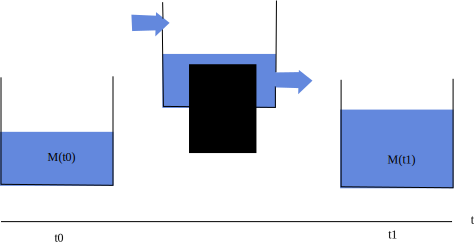
\includegraphics[scale=0.5]{images/continuum_mechanics/massConservation.png}
\caption[STAR mechanics: Mass conservation]{\label{fig:massConservation} Mass conservation. $M(t_{1}) = M(t_{0}) + M_{added} + M_{removed}$}
\end{figure}

The conservation of mass is quite explicit. Mass cannot be created or destroyed. If we look at a small volume $\mathcal{V}$ of the domain $\Omega$, the variation of mass in $\mathcal{V}$ should be equal to the flux of mass going through the border of the volume.
\begin{equation}
    \label{eq:massConservation}
    \frac{d}{dt}\left( \int_{\mathcal{V}} \rho dx \right)
    =
    - \int_{\mathcal{\partial V}}\rho \mathbf{v} \cdot \mathbf{n} ds
\end{equation}

From Stokes' formula, we have

\begin{equation}
\int_{\partial \mathcal{V}} \rho \cdot \mathbf{v} \mathbf{n} ds =
\int_{\mathcal{V}} \nabla \cdot \left( \rho \mathbf{v} \right)
\end{equation}

then the conservation of mass can be rewritten as

\begin{equation}
\int_{\mathcal{V}} \frac{d}{dt} \rho + \nabla \cdot \left( \rho  \mathbf{v} \right) dx = 0
\end{equation}

\subsubsection{Conservation of momentum}

\begin{figure}[!ht]
\centering
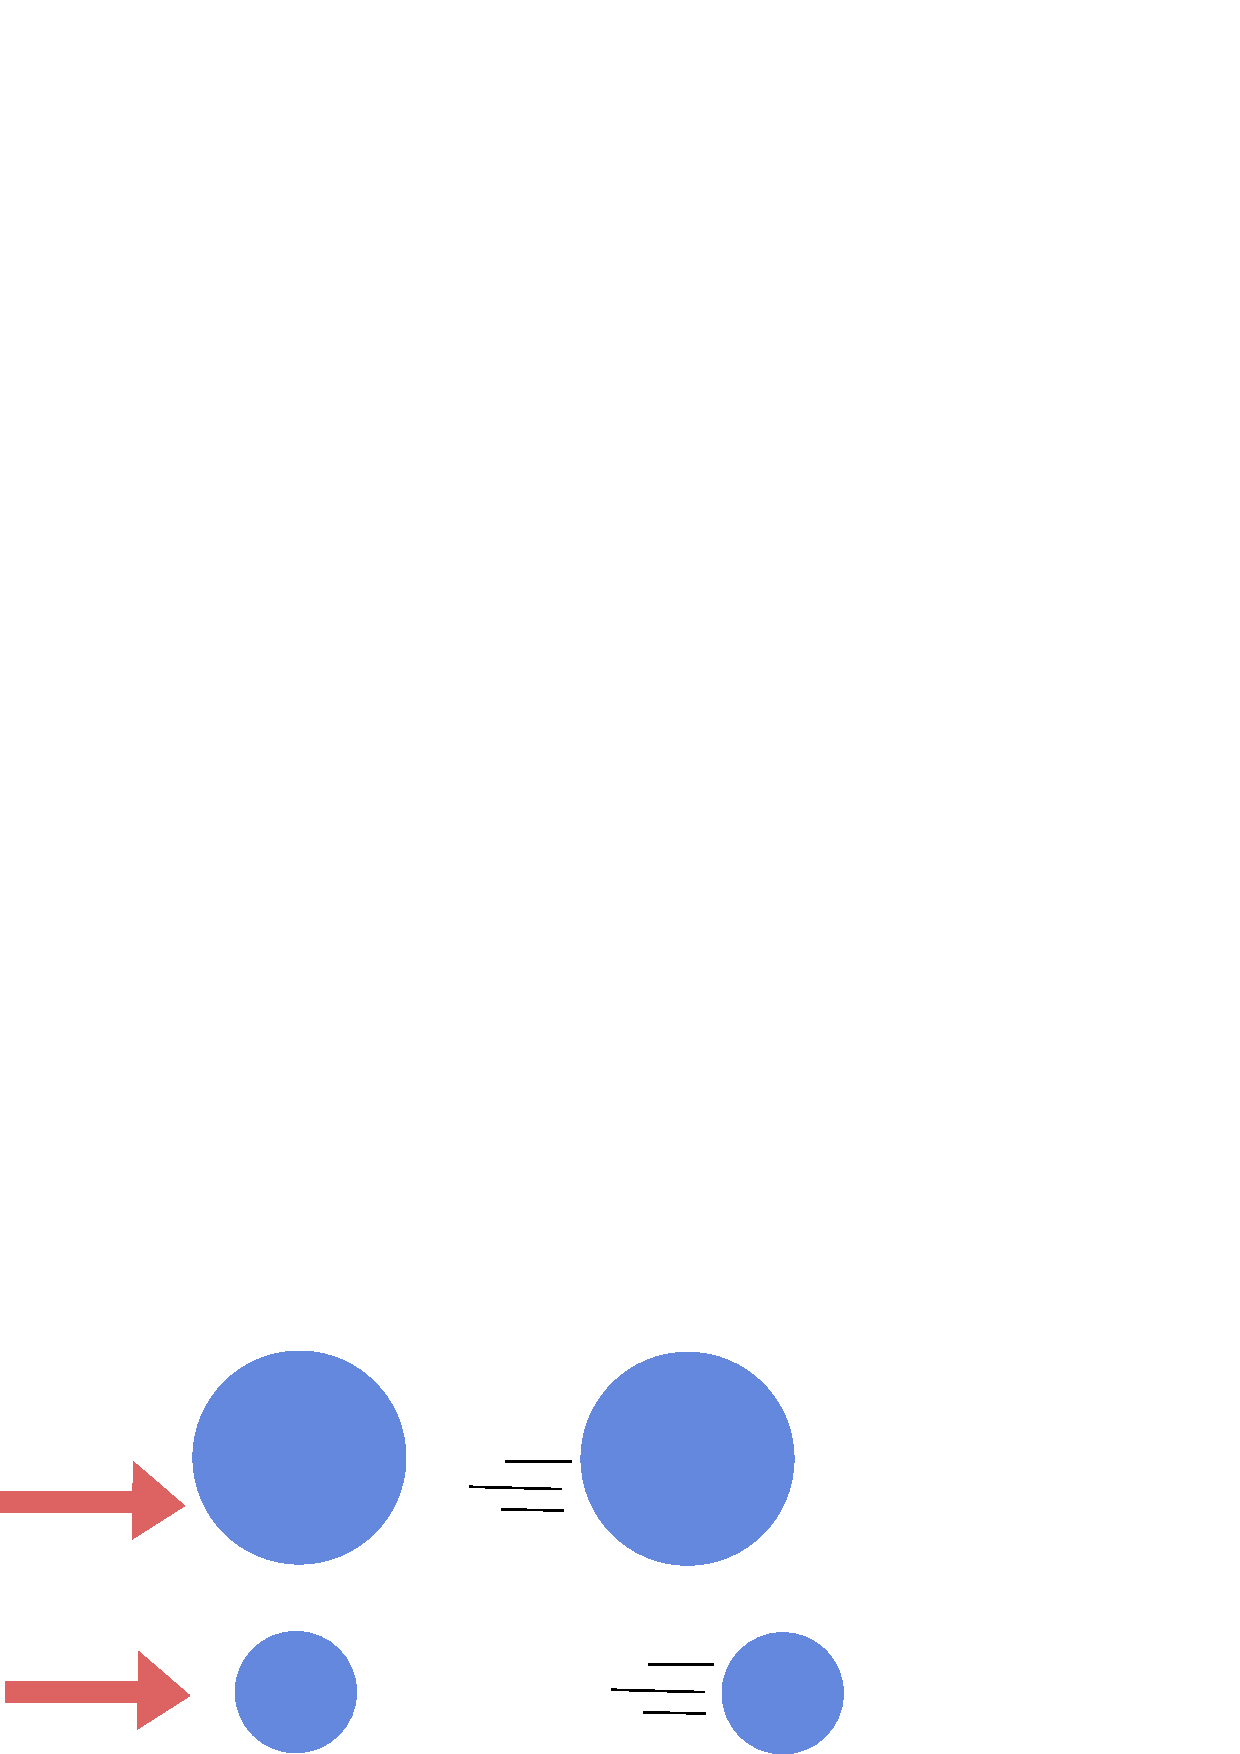
\includegraphics[scale=0.5]{images/continuum_mechanics/momentumConservation.png}
\caption[STAR mechanics: Momentum conservation]{\label{fig:momentumConservation} Momentum conservation.}
\end{figure}

Also called Newton's second law, it states:
\begin{equation}
\label{eq:momentumConservation}
\int_{\mathcal{V}} \rho \frac{D}{Dt} \mathbf{v}(t,x) dx = \int_{V} \mathbf{f} dx
\end{equation}

Two kind of forces are generally applied on an object, the \emph{external} forces and the \emph{internal} forces.

External forces describe the action of the surrounding environment on the object, the simplest example is the gravity:
\begin{equation}
\int_{\mathcal{V}} \rho \mathbf{g} dx
\end{equation}

Internal forces describe the reaction of the object to an external deformation. A general way to describe them is by using a tensor notation:
\begin{equation}
\int_{\mathcal{V}} \sigma \mathbf{n} ds
\end{equation}
By applying the Stokes' formula we can describe it with respect to the volume:
\begin{equation}
\int_{\mathcal{V}} \sigma \mathbf{n} ds =
\int_{\mathcal{V}} \nabla \cdot \sigma dx
\end{equation}

Conservation of momentum can then be rewritten:
\begin{equation}
\int_{\mathcal{V}} \rho \frac{D}{Dt} \mathbf{v}(t,x) dx = \int_{V} \rho \mathbf{g} + \nabla. \sigma dx
\end{equation}

\subsubsection{Lagrangian vs. Eulerian}

\begin{figure}[!ht]
\centering
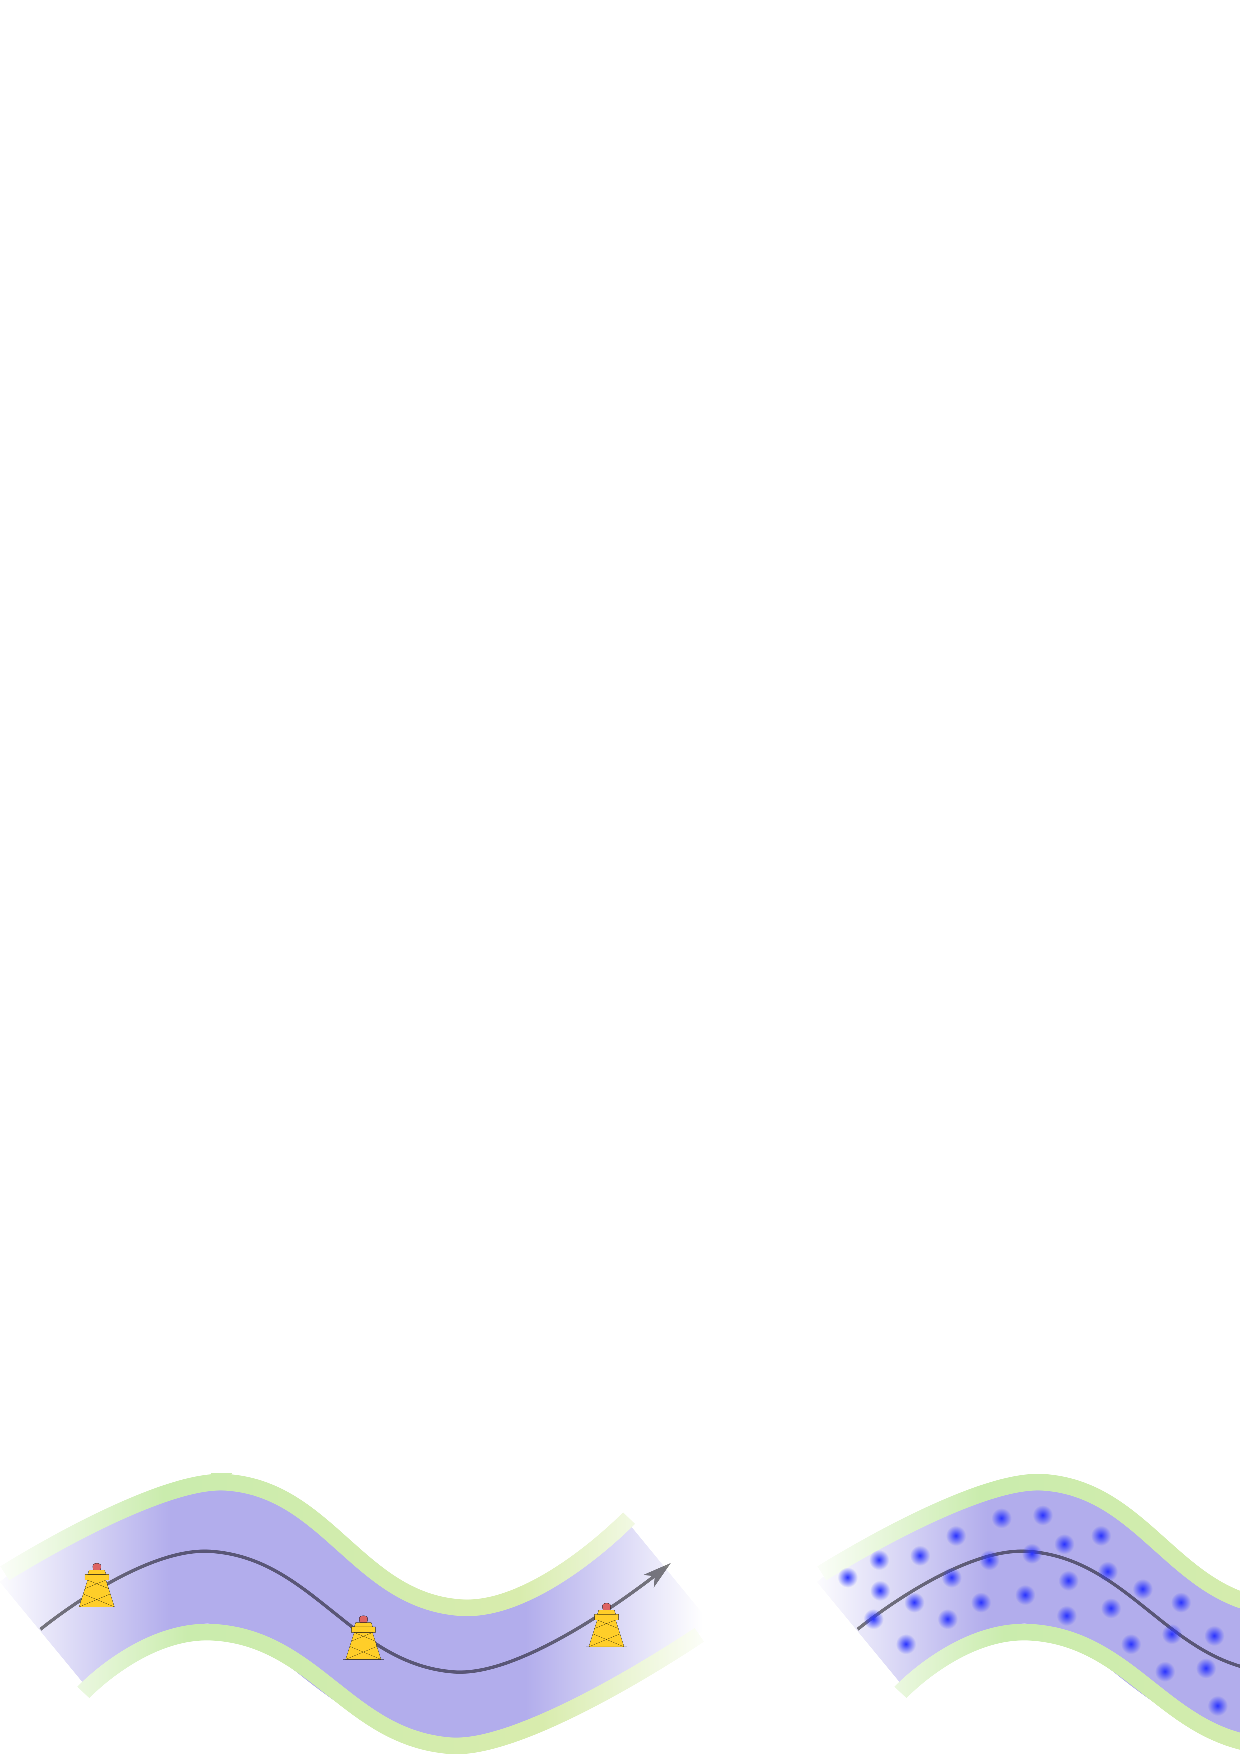
\includegraphics[scale=0.5]{images/continuum_mechanics/eulerianVsLagrangian.png}
\caption[STAR mechanics: Eulerian vs. Lagrangian]{\label{fig:eulerianVsLagrangian} Eulerian vs. Lagrangian viewpoint}
\end{figure}

Lagrangian: You follow the river. The river is discretized into particles which carries and update fluid properties such as position and velocity. 

Eulerian : You stand in the middle of a river. The river is discretized into a fixed grid from where you can measure the velocity of the flow passing through the point of the grid.

The material derivative:
\begin{equation}
\frac{D\mathbf{u}}{Dt} = \frac{\partial \mathbf{u}}{\partial t} + (\mathbf{u} \cdot \nabla v)
\end{equation}

In a lagrangian framework, the positions of the particles at a specific time $t$ is known, so the material derivative is just the time derivative.

\begin{equation}
\frac{D\mathbf{u}}{Dt} = \frac{\partial u}{\partial t}
\end{equation}

Moreover, if we assume that the mass of the particles is constant through the simulation, then conservation of mass is granted and we can omit its numerical solving. However, in practice it does not ensure that the divergence of the velocity will be null, new methods were proposed to enforce the null divergence condition. In this work we keep the first approximation and do not enforce the null divergence condition.

\subsubsection{Spatial discretization}

In order to solve for the equations of motion, we need three ingredients:
\begin{itemize}
\item Degrees of freedom to discretize the equations of motion.
\item An interpolation method to approximate the continuous field discretized on the degrees of freedom.
\item An integration method to integrate data over the whole object.
\end{itemize}

\paragraph{Degrees of freedom}
\begin{itemize}
\item Points
\item Frame
\end{itemize}

\paragraph{Interpolation}

Spatial discretization are divided into two categories: mesh-based and meshfree. For both of them, different kind of degrees of freedom can be chosen. For both of them, different interpolation methods can be chosen. 

\begin{itemize}
\item Mesh-based interpolation
\begin{itemize}
\item Bilinear interpolation
\item Barycentric interpolation
\end{itemize}
\item Mesh-less interpolation
\begin{itemize}
\item SPH interpolation
\item Voronoi interpolation
\end{itemize}
\end{itemize}

\paragraph{Integration}

\begin{itemize}
\item Midpoint rule
\end{itemize}

\subsubsection{Temporal integration}

\paragraph{Explicit}
\begin{itemize}
\item Easy to discretize, implement
\item Stability might be an issue
\end{itemize}

\paragraph{Implicit}
\begin{itemize}
\item Harder to implement
\item Unconditionally stable
\end{itemize}

\subsection{Fluid mechanics}

\subsubsection{Constitutive Law}

Fluid may be subject to an additional constraint whether they are incompressible or not. Incompressibility states that the mass should not vary over time. Then the mass conservation can be rewritten as:
\begin{equation}
\nabla \cdot \mathbf{v} = 0
\end{equation}

For an incompressible fluid, the fluid reacts to pressure and viscosity and thus the constitutive law can be written as:
\begin{equation}
\sigma = -pI + \eta \left( \nabla \mathbf{v} + \nabla \mathbf{v}^{T} \right)
\end{equation}

Then we have:
\begin{equation}
\nabla \cdot \sigma = \nabla \cdot \left( -pI + \eta \left( \nabla \mathbf{v} + \nabla \mathbf{v}^{T} \right) \right) = -\nabla p + \Delta \mathbf{v}
\end{equation}

With internal forces, we have the Navier-Stokes equation for an incompressible fluid:

\begin{equation}
\begin{array}{ll}
\displaystyle
\int_{\mathcal{V}} \rho \frac{D}{Dt} \mathbf{v}(t,x) dx = \int_{V} \rho \mathbf{g} -\nabla p + \eta \Delta \mathbf{v} dx \\ \\
\displaystyle
\nabla. \mathbf{v} = 0
\end{array}
\end{equation}

\subsubsection{SPH model}
Smoothed Particles Hydrodynamics is an interpolation method that can be used to discretize the Navier-Stokes equation in a Lagrangian way. The fluid is discretized into particles which represent a small volume of the whole fluid and each quantity is interpolated using SPH.

\paragraph{SPH interpolation}
The interpolation of a function $f$ at a position $\mathbf{x}$ is :
\begin{equation}
f(\mathbf{x}) = \int_{V} f(\mathbf{x'})W(\mathbf{x}-\mathbf{x'}, h)dx'
\end{equation}
where $W$ is a function called \emph{kernel}. 

If the fluid is discretized into particles with a mass $m$, a density $\rho$ and a volume $V$, then we can discretize the SPH interpolation as:
\begin{equation}
f(\mathbf{x}) = \sum_{p} f(\mathbf{x}_{p})V_{p} W(\mathbf{x}-\mathbf{x_{p}},h) = \sum_{p} f(\mathbf{x}_{p})\frac{m_{p}}{\rho_{p}} W(\mathbf{x}-\mathbf{x_{p}},h)
\end{equation}

Then derivatives can be computed and discretized the same way:
\begin{equation}
D^{\alpha} f(\mathbf{x}) = \int_{\mathcal{V}} f(\mathbf{x'}) D^{\alpha} W(\mathbf{x}-\mathbf{x'}, h)dx'
\end{equation}

\begin{equation}
D^{\alpha} f(\mathbf{x})= \sum_{p} f(\mathbf{x}_{p})\frac{m_{p}}{\rho_{p}} D^{\alpha} W(\mathbf{x}-\mathbf{x_{p}},h)
\end{equation}

However, for first derivatives, the approximation does not vanish if $f$ is constant. A quick way to ensure that is to use a differentiable function $\Phi$ (in practice we use the density $\rho$) to re-write the derivative using the derivative of a product :
\begin{equation}
\nabla f(x) = \frac{1}{\Phi}\left(\nabla (f \Phi) - f \nabla \Phi \right)
\end{equation}

\paragraph{How to choose the kernel}
The properties of $W$ can vary with respect to the properties of the function to be interpolated. In general, $W$ meet the following properties:
\begin{itemize}
\item $W$ is normalized. Thus, constants are interpolated exactly.
\item $W$ has a compact support.
\begin{equation}
\parallel \mathbf{x} \parallel \geq h \rightarrow W(\mathbf{x},h) = 0 
\end{equation}
\begin{equation}
\int_{\mathcal{V}} W(\mathbf{x},h) dx = 1
\end{equation}
\item $W$ tend to the delta function when the length scale $h$ tends to $0$.
\begin{equation}
\lim_{h \rightarrow 0} W(x,h) = \delta(x)
\end{equation}
\item $W$ should be symmetric to enforce invariance under rotation
\begin{equation}
W(-x,h) = W(x,h)
\end{equation}
\item Depending on the function to interpolate the kernel should be positive to prevent unphysical interpolated value.
\begin{equation}
W \geq 0
\end{equation}
\end{itemize}

The cubic kernel from Monaghan is a good choice in practice.

\paragraph{Applications to Navier-Stokes}

\begin{equation}
\rho_{i} = \sum_{j} m_{j}W(\mathbf{x_{j}}-\mathbf{x_{j}},h)
\end{equation}

\begin{equation}
\left(\nabla p\right)_{i} = \sum_{j} \frac{m_{j}}{\rho_{j}} p_{j} \nabla W(\mathbf{x_{j}}-\mathbf{x_{j}},h)
\end{equation}

However linear and angular momentum are not conserved as the formula is not symmetric. By using the previous technique with $\Phi = \frac{1}{\rho}$, it can be symmetrized:

\begin{equation}
\left(\nabla p\right)_{i} = 
\frac{1}{\rho_{i}}
\sum_{j} m_{j} \left( \frac{p_{i}}{\rho_{i}^{2}} + \frac{p_{j}}{\rho_{j}^{2}} \right) \nabla W(\mathbf{x_{j}}-\mathbf{x_{j}},h)
\end{equation}

\begin{equation}
\left(\Delta \mathbf{v}\right)_{i} = \sum_{j} \frac{m_{j}}{\rho_{j}} \mathbf{v}_{j} \Delta W(\mathbf{x_{j}}-\mathbf{x_{j}},h)
\end{equation}

Same as for the pressure gradient, this is not symmetric. Here it can be symmetrized by using $\Phi = \rho$.

\begin{equation}
\left(\Delta \mathbf{v}\right)_{i} = \frac{1}{\rho_{i}}\sum_{j} m_{j} \left( \mathbf{v}_{j}-\mathbf{v}_{i}\right) \Delta W(\mathbf{x_{j}}-\mathbf{x_{j}},h)
\end{equation}

In practice, the evaluation of the laplacian is not accurate. Another form of viscosity based on the gradient was proposed. This is still an area of research.

\begin{equation}
\left(\Delta v\right)_{i} = 
\frac{1}{\rho_{i}}
\sum_{j} m_{j} \Pi_{ij} \nabla W(\mathbf{x_{j}}-\mathbf{x_{j}},h)
\end{equation}

where 

\begin{equation}
\Pi_{ij} = -\frac{2hc_{s}}{\rho_{i}+\rho_{j}}\frac{v_{ij}^{T}x_{ij}}{\vert x_{ij} \vert^{2} + \epsilon h^{2}}
\end{equation}

Now if we discretize Navier-Stokes for one particle $i$, we have:

\begin{equation}
m_{i}\frac{d}{dt}\mathbf{v}_{i}(t) = m_{i}\mathbf{g} - m_{i}(\nabla p)_{i} + m_{i}(\delta \mathbf{v})_{i}
\end{equation}

This equation can now be discretized in time and integrated. In practice we use the euler symplectic integrator:

\begin{equation}
\begin{array}{ll}
\displaystyle \mathbf{v}_{i}(t+\Delta t) = \mathbf{v}_{i}(t) + \Delta t \frac{d}{dt}\mathbf{v}_{i}(t) \\ \\
\displaystyle \mathbf{x}_{i}(t+\Delta t) = \mathbf{x}_{i}(t) + \Delta t \mathbf{v}_{i}(t+\Delta t)
\end{array}
\end{equation}

Several interesting implementation problems arise when dealing with particle system and more particularly particle-based fluid simulations:

\begin{itemize}
\item Boundary handling 
\item Surface reconstruction
\item Optimization (acceleration structure for spatial query)
\end{itemize}

Faire un tableau avec les références et ce que l'on peut y trouver d'intéressant.

%\paragraph{Eulerian grid}
%\paragraph{Lagrangian particles}
%\paragraph{Hybrid method}
%\paragraph{Smoothed Hydrodynamics Particles model}

\subsection{Solid mechanics}

\subsubsection{Constitutive Law}
A common way to describe the stress tensor for elastic materials is to use a constitutive density energy:
\begin{equation}
\sigma = \frac{\partial \Psi}{\partial \epsilon}
\end{equation}

There are many forms of enery. For a classical Hookean material, the density energy is
\begin{equation}
\Psi = \frac{1}{2}H\epsilon^{2}
\end{equation}

Then the stress tensor is
\begin{equation}
\sigma = H\epsilon
\end{equation}

H is called the stiffness tensor and is a $3\times3\times3\times3$ tensor. For isotropic materials, the number of material parameters can be reduced to two, the Young's modulus $E$ and the Poisson's ratio $\nu$. Also, the strain and stress tensor being symmetric, the constitutive law can be simplified:
\begin{equation}
\sigma = 
\begin{bmatrix}
\sigma_{11} \\
\sigma_{22} \\
\sigma_{33} \\
\sigma_{23} \\
\sigma_{13} \\
\sigma_{12}
\end{bmatrix}
=
\tilde{H}
\begin{bmatrix}
\epsilon_{11} \\
\epsilon_{22} \\
\epsilon_{33} \\
2\epsilon_{23} \\
2\epsilon_{13} \\
2\epsilon_{12}
\end{bmatrix}
\end{equation}

where

\begin{equation}
\tilde{H} =
\frac{E}{\left(1+\nu\right)\left(1-2\nu\right)}
\begin{bmatrix}
1-\nu & \nu & \nu & 0 & 0 & 0 \\ 
\nu & 1-\nu & \nu & 0 & 0 & 0 \\
\nu & \nu & 1-\nu & 0 & 0 & 0 \\
0 & 0 & 0 & \frac{1-2\nu}{2} & 0 & 0 \\
0 & 0 & 0 & 0 & \frac{1-2\nu}{2} & 0 \\
0 & 0 & 0 & 0 & 0 & \frac{1-2\nu}{2} \\
\end{bmatrix}
\end{equation}

The strain is used to measure the relative deformation with respect to the rest position of the object: elongation, compression. Therefore it is  linked to the variation of position of the object. In 3D, this position is described by 3 coordinates which can be derived with respect to each direction, then the strain should be represented by a $3\times3$ matrix.

An object is deformed if it has been compressed, stretched or sheared. The strain should measure this deformation and be $0$ when the object is at its rest position. This constraint can be expressed as:
\begin{equation}
\epsilon = \mathbf{F}^{T}\mathbf{F}-I
\end{equation}

where $F$ is called the deformation gradient:
\begin{equation}
\mathbf{F} = \frac{\partial \Phi}{\partial \mathbf{x_{0}}}
\end{equation}

and $\Phi$ is the displacement field, the mapping between the rest shape $\Omega_{0}$ and the deformed shape of the object $\Omega$. 

\begin{equation}
\begin{array}{llll}
\Phi & \Omega_{0} & \longrightarrow & \Omega \\
	 & \mathbf{x_{0}} & \longrightarrow & \mathbf{x}
\end{array}
\end{equation}

For elastic object, as the position is always relative to the rest position, it can be written using a displacement vector:
\begin{equation}
\Phi(\mathbf{x_{0}}) = \mathbf{x}_{0} + \mathbf{u}
\end{equation}

Then the strain relation becomes
\begin{equation}
\epsilon = \nabla \mathbf{u} + \left( \nabla \mathbf{u} \right)^{T} + \left(\nabla \mathbf{u}\right)^{T}\nabla \mathbf{u}
\end{equation}

It is called the Green-Lagrange strain and its linearized version the Cauchy strain.

\begin{equation}
\epsilon = \nabla \mathbf{u} + \left( \nabla \mathbf{u} \right)^{T}
\end{equation}

The strain measurement is the big difference with respect to fluid dynamics because it is the link between the deformed object and its rest shape whereas there are no such thing when computing the stress for a fluid.

\subsubsection{Frame-based model}

\paragraph{Degrees of freedom}
The object is uniformly sampled with affine frames as degrees of freedom. Affine frames $T=(A,t)$ represent $12$ degree of freedoms, $3$ for translation $\mathbf{t}$, $9$ for the matrix $\mathbf{A}$ combining rotation, scaling and shearing. Affine frames are represented with respect to an initial configuration $T_{0} = \left(A_{0}, t_{0}\right)$.

\paragraph{Interpolation}
Linear blend skinning is used to interpolate the displacement field. A deformed position $\mathbf{x}$ can be interpolated as a weighted sum of the affine transformations applied to the rest position $\mathbf{x_{0}}$.

\begin{equation}
\mathbf{x} = \sum_{i} w_{i}(\mathbf{x_{0}})\left(t_{i}+A_{i}\mathbf{x_{0}^{rel}}\right)
\end{equation}

where $\mathbf{x_{0}^{rel}}$ is the relative position of $x_{0}$ in the frame defined by $T_{0}$, in other words:

\begin{equation}
\mathbf{x_{0}}^{rel} = A_{0}^{-1}\left( \mathbf{x_{0}} - \mathbf{t_{0}} \right)
\end{equation}

Deformation gradient can then be easily derived:
\begin{equation}
F = \frac{\partial \mathbf{x}}{\partial \mathbf{x_{0}}} =
\nabla w_{i}(\mathbf{x_{0}}) \left( t_{i}+A_{i}x_{0}^{rel}\right) + 
w_{i}\left( A_{i}A_{0}^{-1} \right)
\end{equation}

\paragraph{Voronoi shape function}

Different weights can be used. Three properties are important in order to represent a physical behavior:

\begin{itemize}
\item Weights should linearly decrease with respect to distance in the material.
\item Weights should be positive.
\item Weights should form a partition of unity.
\end{itemize}

\begin{itemize}
\item Description du calcul des poids
\end{itemize}

\paragraph{Spatial integration}

Any quadrature rule can be used. Here, for the sake of simplicity, we suppose that the integration points are collocated with the frames and that we use the midpoint rule. Thus, the integral of a function $f$ over the object states:
\begin{equation}
\int_{V} f(x)  = \sum_{i} V_{i} f(x_{i})
\end{equation}

Let's describe how internal forces are computed. A nice way to compute the forces is to decompose its energy formulation.
\begin{equation}
\mathbf{f} = - \int_{V} \left( \frac{\partial \Psi}{\partial \mathbf{x}} \right)^{T} =
- \int_{V} 
\left( \frac{\partial \mathbf{F}}{\partial \mathbf{x}} \right)^{T}
\left( \frac{\partial \epsilon}{\partial \mathbf{F}} \right)^{T}
\left( \frac{\partial \Psi}{\partial \mathbf{\epsilon}} \right)^{T}
\end{equation}
Thus we decomposed the computation with respect to the different mappings involved in a physical system:
\begin{itemize}
\item The deformation gradient mapping $F$.
\item The strain mapping $\epsilon$.
\item The energy mapping $\psi$.
\end{itemize}

Thus, the internal force on one frame $f_{i}$ are:
\begin{equation}
f_{i} = - \sum_{i} V_{i} \left( \frac{\partial \mathbf{F}}{\partial \mathbf{x}} \right)^{T}
\left( \frac{\partial \epsilon}{\partial \mathbf{F}} \right)^{T}
\left( \frac{\partial \Psi}{\partial \mathbf{\epsilon}} \right)^{T}
\end{equation}

\begin{itemize}
\item Partir de l'hypothèse d'un point d'intégration par région de voronoi.
\item Décrire le calcul des forces de manière généralisée.
\end{itemize}

Each term can be computed in a separate dedicated module with its own rules, type and resolution.

\paragraph{Temporal integration}

This needs to be developed.
Also, the mass matrix computation should be described.
\begin{equation}
\begin{array}{l}
t(t+\Delta t) = t(t) + \frac{1}{m_{i}}f(t) \\ \\
A(t+\Delta t) = A(t) + I(t)\tau(t)
\end{array}
\end{equation}

where $I(t)$ is the inertia tensor:

\begin{equation}
I(t) = M^{-1}(t) = R(t)M(t)R(t)^{T} 
\end{equation}

\paragraph{Multi-layer physical framework}

\begin{itemize}
\item Common components in simulation framework
\item Lack of usability
\item Lack of modularity
\item Lack of granularity
\item A solution: layering
\end{itemize}

Four different layers are used in the frame-based framework.
\begin{itemize}
\item Degrees of freedom layer
\item Integration layer
\item Visualization layer
\item Collision layer
\end{itemize}

Each of them communicates using mapping.
It allows an easier repartition of resources and computational task.

Sujets non évoqués:
\begin{itemize}
\item Collision detection and response
\item Strain rate (viscosity)
\end{itemize}

%\section[A quick \& dirty introduction to fluid dynamics]{A quick \& dirty introduction to computational fluid dynamics}
%
%\subsection{Navier-Stokes equation}
%
%\paragraph{Mass conservation}
%The conservation of mass is quite explicit. The mass of the fluid cannot change. Mathematically, it is expressed by stating that the variation of the mass in a given volume is equal to the flux of mass going through the border of the volume.
%\begin{equation}
%    \label{eq:massConservation}
%    \frac{d}{dt}\left( \int_{\mathcal{V}} \rho dx \right)
%    =
%    - \int_{\mathcal{\partial V}}\rho \mathbf{v} \mathbf{n} ds
%\end{equation}
%
%From Stokes' formula, we have
%
%\begin{equation}
%\int_{\partial \mathcal{V}} \rho \mathbf{v} \mathbf{n} ds =
%\int_{\mathcal{V}} \nabla \cdot \left( \rho \mathbf{v} \right)
%\end{equation}
%
%then the conservation of mass can be rewritten as
%
%\begin{equation}
%\int_{\mathcal{V}} \frac{d}{dt} \rho + \nabla \cdot \left( \rho  \mathbf{v} \right) dx = 0
%\end{equation}
%
%\paragraph{Constitutive Law}
%The constitutive law describes how the fluid react to a deformation. For an incompressible fluid, the fluid reacts to pressure and viscosity and can be written:
%\begin{equation}
%\sigma = -pI + \eta \left( \nabla \mathbf{v} + \nabla \mathbf{v}^{T} \right)
%\end{equation}
%
%\paragraph{Incompressibility}
%This states that the mass should not vary over time. Then the mass conservation can be rewritten as:
%\begin{equation}
%\nabla \cdot u = 0
%\end{equation}
%
%\paragraph{Momentum conservation}
%
%Also called Newton's second law, it states:
%\begin{equation}
%\label{eq:momentumConservation}
%\int_{\mathcal{V}} \rho \frac{D}{Dt} \mathbf{v}(t,x) dx = \int_{V} \mathbf{f} dx
%\end{equation}
%
%Two kind of forces are generally applied on a fluid, the \emph{external} forces and the \emph{internal} forces.
%
%External forces describe the action of the surrounding environment on the fluid, the simplest example is the gravity:
%\begin{equation}
%\int_{\mathcal{V}} \rho \mathbf{g} dx
%\end{equation}
%
%Internal forces describe the reaction of the fluid to an external deformation. A general way to describe them is by using a tensor notation:
%\begin{equation}
%\int_{\mathcal{V}} \sigma \mathbf{n} ds
%\end{equation}
%By applying the Stokes' formula we can describe it with respect to the volume:
%\begin{equation}
%\int_{\mathcal{V}} \sigma \mathbf{n} ds =
%\int_{\mathcal{V}} \nabla \cdot \sigma dx
%\end{equation}
%
%Conservation of momentum can then be rewritten:
%\begin{equation}
%\int_{\mathcal{V}} \rho \frac{D}{Dt} \mathbf{v}(t,x) dx = \int_{V} \rho \mathbf{g} + \nabla. \sigma dx
%\end{equation}
%
%Then we have:
%\begin{equation}
%\nabla \cdot \sigma = \nabla \cdot \left( -pI + \eta \left( \nabla \mathbf{v} + \nabla \mathbf{v}^{T} \right) \right) = -\nabla p + \Delta \mathbf{v}
%\end{equation}
%
%With internal forces, we have the Navier-Stokes equation for an incompressible fluid:
%
%\begin{equation}
%\begin{array}{ll}
%\int_{\mathcal{V}} \rho \frac{D}{Dt} \mathbf{v}(t,x) dx = \int_{V} \rho \mathbf{g} -\nabla p + \eta \Delta \mathbf{v} dx \\
%\nabla. \mathbf{u} = 0
%\end{array}
%\end{equation}
%
%\paragraph{Lagrangian vs Eulerian}
%
%Lagrangian: You follow the river. The river is discretized into particles which carries and update fluid properties such as position and velocity. 
%
%Eulerian : You stand in the middle of a river. The river is discretized into a fixed grid from where you can measure the velocity of the flow passing through the point of the grid.
%
%The material derivative:
%\begin{equation}
%\frac{D\mathbf{u}}{Dt} = \frac{\partial \mathbf{u}}{\partial t} + (\mathbf{u} \cdot \nabla v)
%\end{equation}
%
%In a lagrangian framework, the positions of the particles at a specific time $t$ is known, so the material derivative is just the time derivative.
%
%\begin{equation}
%\frac{D\mathbf{u}}{Dt} = \frac{\partial u}{\partial t}
%\end{equation}
%
%Moreover, if we assume that the mass of the particles is constant through the simulation, then conservation of mass is granted and we can omit its numerical solving. However, in practice it does not ensure that the divergence of the velocity will be null, new methods were proposed to enforce the null divergence condition. In this work we keep the first approximation and do not enforce the null divergence condition.
%
%\subsection{Discretization}
%
%Once equations of motion have been set, they can be discretized in space and time and integrated.
%
%\subsection{Discretization: The Smoothed Hydrodynamics Particles model}
%Smoothed Particles Hydrodynamics is an interpolation method that can be used to discretize the Navier-Stokes equation in a Lagrangian way. The fluid is discretized into particles which represent a small volume of the whole fluid and each quantity is interpolated using SPH.
%
%\paragraph{SPH interpolation}
%The interpolation of a function $f$ at a position $\mathbf{x}$ is :
%\begin{equation}
%f(\mathbf{x}) = \int_{V} f(\mathbf{x'})W(\mathbf{x}-\mathbf{x'}, h)dx'
%\end{equation}
%where $W$ is a function called \emph{kernel}. 
%
%If the fluid is discretized into particles with a mass $m$, a density $\rho$ and a volume $V$, then we can discretize the SPH interpolation as:
%\begin{equation}
%f(\mathbf{x}) = \sum_{p} f(\mathbf{x}_{p})V_{p} W(\mathbf{x}-\mathbf{x_{p}},h) = \sum_{p} f(\mathbf{x}_{p})\frac{m_{p}}{\rho_{p}} W(\mathbf{x}-\mathbf{x_{p}},h)
%\end{equation}
%
%Then derivatives can be computed and discretized the same way:
%\begin{equation}
%D^{\alpha} f(\mathbf{x}) = \int_{\mathcal{V}} f(\mathbf{x'}) D^{\alpha} W(\mathbf{x}-\mathbf{x'}, h)dx'
%\end{equation}
%
%\begin{equation}
%D^{\alpha} f(\mathbf{x})= \sum_{p} f(\mathbf{x}_{p})\frac{m_{p}}{\rho_{p}} D^{\alpha} W(\mathbf{x}-\mathbf{x_{p}},h)
%\end{equation}
%
%However, for first derivatives, the approximation does not vanish if $f$ is constant. A quick way to ensure that is to use a differentiable function $\Phi$ (in practice we use the density $\rho$) to re-write the derivative using the derivative of a product :
%\begin{equation}
%\nabla f(x) = \frac{1}{\Phi}\left(\nabla (f \Phi) - f \nabla \Phi \right)
%\end{equation}
%
%\paragraph{How to choose the kernel}
%The properties of $W$ can vary with respect to the properties of the function to be interpolated. In general, $W$ meet the following properties:
%\begin{itemize}
%\item $W$ is normalized. Thus, constants are interpolated exactly.
%\item $W$ has a compact support.
%\begin{equation}
%\parallel \mathbf{x} \parallel \geq h \rightarrow W(\mathbf{x},h) = 0 
%\end{equation}
%\begin{equation}
%\int_{\mathcal{V}} W(\mathbf{x},h) dx = 1
%\end{equation}
%\item $W$ tend to the delta function when the length scale $h$ tends to $0$.
%\begin{equation}
%\lim_{h \rightarrow 0} W(x,h) = \delta(x)
%\end{equation}
%\item $W$ should be symmetric to enforce invariance under rotation
%\begin{equation}
%W(-x,h) = W(x,h)
%\end{equation}
%\item Depending on the function to interpolate the kernel should be positive to prevent unphysical interpolated value.
%\begin{equation}
%W \geq 0
%\end{equation}
%\end{itemize}
%
%The cubic kernel from Monaghan is a good choice in practice.
%
%\paragraph{Applications to Navier-Stokes}
%
%\begin{equation}
%\rho_{i} = \sum_{j} m_{j}W(\mathbf{x_{j}}-\mathbf{x_{j}},h)
%\end{equation}
%
%\begin{equation}
%\left(\nabla p\right)_{i} = \sum_{j} \frac{m_{j}}{\rho_{j}} p_{j} \nabla W(\mathbf{x_{j}}-\mathbf{x_{j}},h)
%\end{equation}
%
%However linear and angular momentum are not conserved as the formula is not symmetric. By using the previous technique with $\Phi = \frac{1}{\rho}$, it can be symmetrized:
%
%\begin{equation}
%\left(\nabla p\right)_{i} = 
%\frac{1}{\rho_{i}}
%\sum_{j} m_{j} \left( \frac{p_{i}}{\rho_{i}^{2}} + \frac{p_{j}}{\rho_{j}^{2}} \right) \nabla W(\mathbf{x_{j}}-\mathbf{x_{j}},h)
%\end{equation}
%
%\begin{equation}
%\left(\Delta \mathbf{v}\right)_{i} = \sum_{j} \frac{m_{j}}{\rho_{j}} \mathbf{v}_{j} \Delta W(\mathbf{x_{j}}-\mathbf{x_{j}},h)
%\end{equation}
%
%Same as for the pressure gradient, this is not symmetric. Here it can be symmetrized by using $\Phi = \rho$.
%
%\begin{equation}
%\left(\Delta \mathbf{v}\right)_{i} = \frac{1}{\rho_{i}}\sum_{j} m_{j} \left( \mathbf{v}_{j}-\mathbf{v}_{i}\right) \Delta W(\mathbf{x_{j}}-\mathbf{x_{j}},h)
%\end{equation}
%
%In practice, the evaluation of the laplacian is not accurate. Another form of viscosity based on the gradient was proposed. This is still an area of research.
%
%\begin{equation}
%\left(\Delta v\right)_{i} = 
%\frac{1}{\rho_{i}}
%\sum_{j} m_{j} \Pi_{ij} \nabla W(\mathbf{x_{j}}-\mathbf{x_{j}},h)
%\end{equation}
%
%where 
%
%\begin{equation}
%\Pi_{ij} = -\frac{2hc_{s}}{\rho_{i}+\rho_{j}}\frac{v_{ij}^{T}x_{ij}}{\vert x_{ij} \vert^{2} + \epsilon h^{2}}
%\end{equation}
%
%Now if we discretize Navier-Stokes for one particle $i$, we have:
%
%\begin{equation}
%m_{i}\frac{d}{dt}v_{i}(t) = m_{i}\mathbf{g} - m_{i}(\nabla p)_{i} + m_{i}(\delta \mathbf{v})_{i}
%\end{equation}
%
%This equation can now be discretized in time and integrated. In practice we use the euler symplectic integrator:
%
%\begin{equation}
%\begin{array}{ll}
%v_{i}(t+\Delta t) = v_{i}(t) + \Delta t \frac{d}{dt}v_{i}(t) \\
%x_{i}(t+\Delta t) = x_{i}(t) + \Delta t v_{i}(t+\Delta t)
%\end{array}
%\end{equation}
%
%Several interesting implementation problems arise when dealing with particle system and more particularly particle-based fluid simulations:
%
%\begin{itemize}
%\item Boundary handling 
%\item Surface reconstruction
%\item Optimization (acceleration structure for spatial query)
%\end{itemize}
%
%Faire un tableau avec les références et ce que l'on peut y trouver d'intéressant.
%
%%\paragraph{Eulerian grid}
%%\paragraph{Lagrangian particles}
%%\paragraph{Hybrid method}
%%\paragraph{Smoothed Hydrodynamics Particles model}

%\section[A quick \& dirty introduction to continuum mechanics]{A quick \& dirty introduction to continuum mechanics}

%The behavior of an elastic deformable model is described by conservation laws and a constitutive law.
%
%The first conservation law is the conservation of mass.
%
%The second conservation law is the conservation of momentum.
%
%The constitutive law depict the behavior of the object with respect to a deformation.
%
%\begin{equation}
%\begin{array}{ll}
%\int_{\mathcal{V}} \frac{d\mathbf{v}}{dt} = \int_{\mathcal{V}} \rho \mathbf{g} + \nabla \cdot \sigma dx 
%\\
%\int_{\mathcal{V}} \nabla \cdot u = 0
%\end{array}
%\end{equation} 
%
%A common way to describe the stress tensor for elastic materials is to use a constitutive density energy:
%\begin{equation}
%\sigma = \frac{\partial \Psi}{\partial \epsilon}
%\end{equation}
%
%There are many forms of enery. For a classical Hookean material, the density energy is
%\begin{equation}
%\Psi = \frac{1}{2}H\epsilon^{2}
%\end{equation}
%
%Then the stress tensor is
%\begin{equation}
%\sigma = H\epsilon
%\end{equation}
%
%H is called the stiffness tensor and is a $3\times3\times3\times3$ tensor. For isotropic materials, the number of material parameters can be reduced to two, the Young's modulus $E$ and the Poisson's ratio $\nu$. Also, the strain and stress tensor being symmetric, the constitutive law can be simplified:
%\begin{equation}
%\sigma = 
%\begin{bmatrix}
%\sigma_{11} \\
%\sigma_{22} \\
%\sigma_{33} \\
%\sigma_{23} \\
%\sigma_{13} \\
%\sigma_{12}
%\end{bmatrix}
%=
%\tilde{H}
%\begin{bmatrix}
%\epsilon_{11} \\
%\epsilon_{22} \\
%\epsilon_{33} \\
%2\epsilon_{23} \\
%2\epsilon_{13} \\
%2\epsilon_{12}
%\end{bmatrix}
%\end{equation}
%
%where
%
%\begin{equation}
%\tilde{H} =
%\frac{E}{\left(1+\nu\right)\left(1-2\nu\right)}
%\begin{bmatrix}
%1-\nu & \nu & \nu & 0 & 0 & 0 \\ 
%\nu & 1-\nu & \nu & 0 & 0 & 0 \\
%\nu & \nu & 1-\nu & 0 & 0 & 0 \\
%0 & 0 & 0 & \frac{1-2\nu}{2} & 0 & 0 \\
%0 & 0 & 0 & 0 & \frac{1-2\nu}{2} & 0 \\
%0 & 0 & 0 & 0 & 0 & \frac{1-2\nu}{2} \\
%\end{bmatrix}
%\end{equation}
%
%The strain is used to measure the relative deformation with respect to the rest position of the object: elongation, compression. Therefore it is  linked to the variation of position of the object. In 3D, this position is described by 3 coordinates which can be derived with respect to each direction, then the strain should be represented by a $3\times3$ matrix.
%
%An object is deformed if it has been compressed, stretched or sheared. The strain should measure this deformation and be $0$ when the object is at its rest position. This constraint can be expressed as:
%\begin{equation}
%\epsilon = \left( \nabla \mathbf{x} \right)^{T} \nabla \mathbf{x} - I
%\end{equation}
%
%$\nabla \mathbf{x}$ is also called deformation gradient.
%
%For elastic object, the position is always relative to the rest position. Therefore, a displacement vector is often used to depict the current position.
%\begin{equation}
%\mathbf{x} = \mathbf{x}_{0} + \mathbf{u}
%\end{equation}
%
%Then the strain relation becomes
%\begin{equation}
%\epsilon = \nabla \mathbf{u} + \left( \nabla \mathbf{u} \right)^{T} + \left(\nabla \mathbf{u}\right)^{T}\nabla \mathbf{u}
%\end{equation}
%
%It is called the Green-Lagrange strain and its linearized version the Cauchy strain.
%
%\begin{equation}
%\epsilon = \nabla \mathbf{u} + \left( \nabla \mathbf{u} \right)^{T}
%\end{equation}
%
%The strain measurement is the big difference with respect to fluid dynamics because it is the link between the deformed object and its rest shape whereas there are no such thing when computing the stress for a fluid.
%
%Now we are ready to discretize the equations of motion in space and time.
%
%\paragraph{Discretization}
%
%Now that we have a clear description of the equation of motions, we can discretize them in space and time. Here a large number of methods can be used. 
%
%Spatial discretization are divided into two categories: mesh-based and meshfree. For both of them, different kind of degrees of freedom can be chosen. For both of them, different interpolation methods can be chosen. 
%
%Here we focus on a method called the frame-based model. The degrees of freedom are affine frames and the interpolation method is based on a method called linear blend skinning.
%
%Affine frames represent $9$ degree of freedoms, $3$ for translation, $3$ for rotation and $3$ for scaling. They uniformly sample the object and are used to compute the dynamics.
%
%For elastic objects, we need to build a mapping between the rest shape $\Omega_{0}$ and the deformed shape of the object $\Omega$ in order to compute the deformation gradient, this is called the displacement field $\Phi$.
%
%\begin{equation}
%\begin{array}{llll}
%f & \Omega_{0} & \longrightarrow & \Omega \\
%	 & \mathbf{x_{0}} & \longrightarrow & \mathbf{x}
%\end{array}
%\end{equation}
%
%In order to approximate this mapping, we use a set of functions called the shape functions $\left\lbrace \Phi \right\rbrace_{i}$. This set of functions should be consistent, i.e form a partition of unity :
%\begin{equation}
%f(\mathbf{x}) = \sum_{i} \Phi_{i}(\mathbf{x}) f(\mathbf{x}_{i})
%\end{equation}
%
%For derivatives, computation becomes straightforward:
%\begin{equation}
%D^{\alpha}f(\mathbf{x}) = \sum_{i} D^{\alpha}\Phi_{i}(\mathbf{x}) f(\mathbf{x}_{i})
%\end{equation}
%
%\begin{itemize}
%\item Collision detection and response
%\item Strain rate (viscosity)
%\end{itemize}
\section{Control of physics-based animation}
\label{sec:starSimulationControl}

As we mentioned in the introduction, computer were used for producing animations in two main ways. 
First, principles of traditional animation were adopted, leaving the animator to describe the key-frames that would bring life and style to characters. 
Second, physics was used to animate objects whose complexity in terms of scale and behavior would have been intractable for a single animator. 
Nowadays, these two use cases are only the extremities of a large spectrum. 
In between lies the control of physics-based animations which tends to take into account both user directions, that will bring life and style, and physics, that will handle the exciting complexity and dynamics of the physical behavior.

\subsection{Problem: The trials and errors process}

How to control a physics-based animation is an old problem in Computer Graphics. In order to understand the different problems that arise, it is good to start from the most naive way of controlling a physics-based animation: trials and errors. 

Let's say we have to design an animation of a ball launched on the ground that bounces two times before hitting the center of a target on the ground. 
The elastic behavior of the ball and the changes of speed make it a hard animation for a key-framing animator. 
Using physically-based simulation methods, the behavior takes some time to compute but can be easily solved.
As the simulation is an initial value problem, the whole behavior of the ball is dictated by the initial and boundary conditions of the simulation, the material parameters of the ball and the \emph{wind} forces that can be set to help guiding the animation. 
The trials and errors process consists in setting these conditions and parameters, running the simulation and correcting the parameters until the ball reaches the desired target (see Figure~\ref{fig:trialErrorProcess}). 
There are mainly two constraints which make this task a nightmare:
\begin{itemize}
	\item Firstly, the computational time plays a major role. 
	This is obvious but still important to states. 
	A real-time simulation will allow the user to quickly explore parameters whereas an offline simulation might require days and days of tuning.
	\item Secondly, the control is indirect and, most of the time, based on unintuitive parameters which requires some expertise about the underlying physical model. The user cannot directly control the trajectory nor the shape of the object.
	\item Thirdly, many physics-based animations describe a non-linear behavior. Fluid animations are among them for instance. 
	This non-linearity makes it very hard to choose the right parameters. 
	Small changes can produce very different results making tedious to explore the range of possible behaviors and almost impossible to respect specific artistic directions such as timing, key positions, trajectories or shapes. 
	Also, it prevents the user from interactively controlling a low-resolution simulation and then achieve a similar behavior with the same parameters at a higher resolution.
\end{itemize}

\begin{figure}[!h]
	\centering
	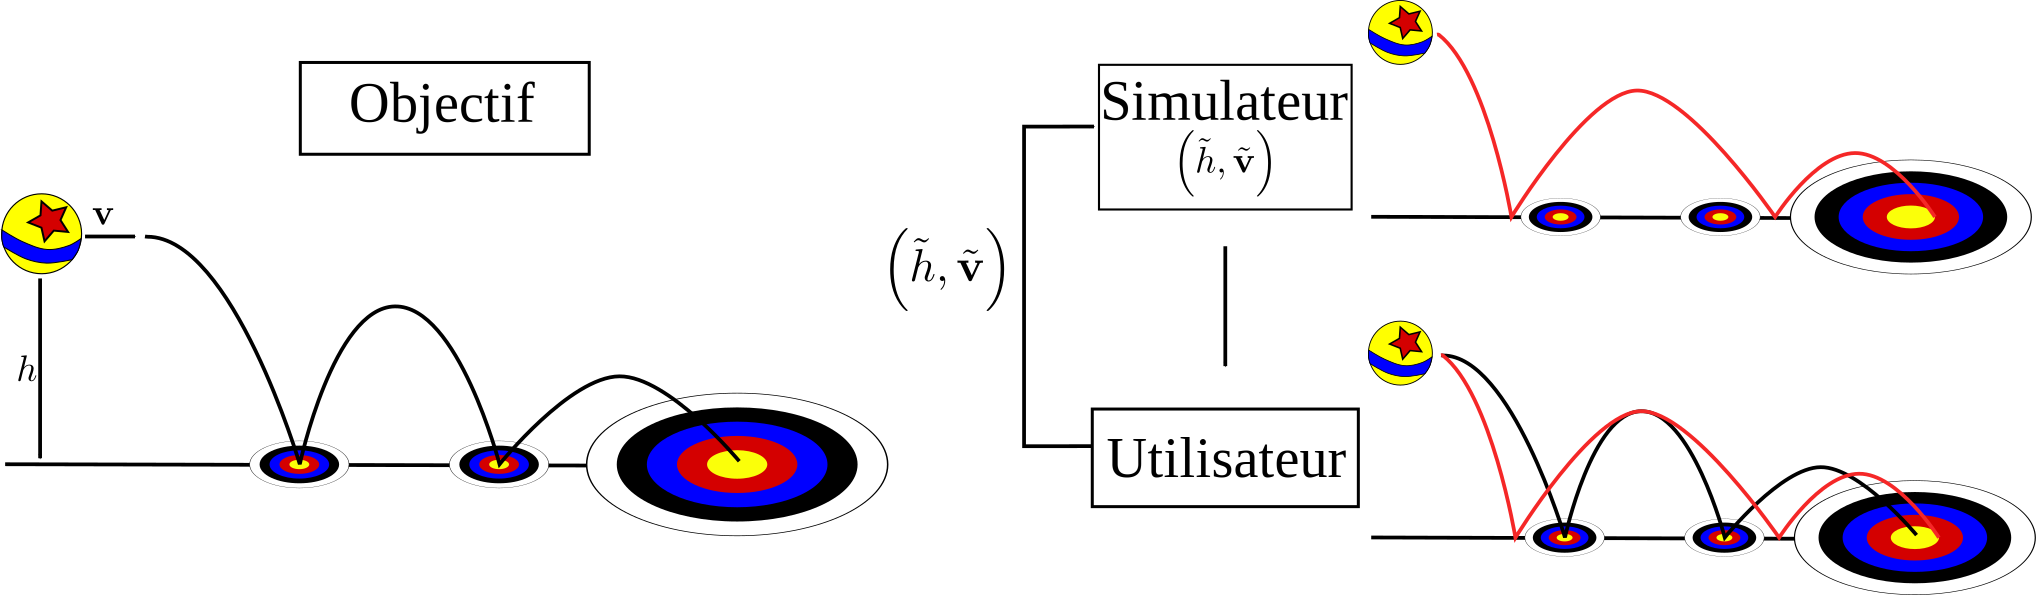
\includegraphics[scale=0.20]{./images/simulationControl/trialError.png}
	\caption[STAR control: Trial and error process]{\label{fig:trialErrorProcess}Trial and error process}
\end{figure}

\subsection{Space-time constraints paradigm}
A general approach for controlling a physics-based animation is to formulate it as an optimization under constraints: 
"\emph{Find the parameters such that the physical behavior and user constraints are respected over the animation}" 
(see Figure~\ref{fig:spaceTimeConstraints}). 
Four challenges arise, what are the parameters we want to control, what are the user constraints, how to formulate them and finally how to numerically solve the problem. 
Witkin and Kass~\cite{Witkin1988} were among the first to introduce this formulation to the Computer Graphics community in their pioneer work \emph{Space-time constraints}.

\begin{figure}[!h]
\centering
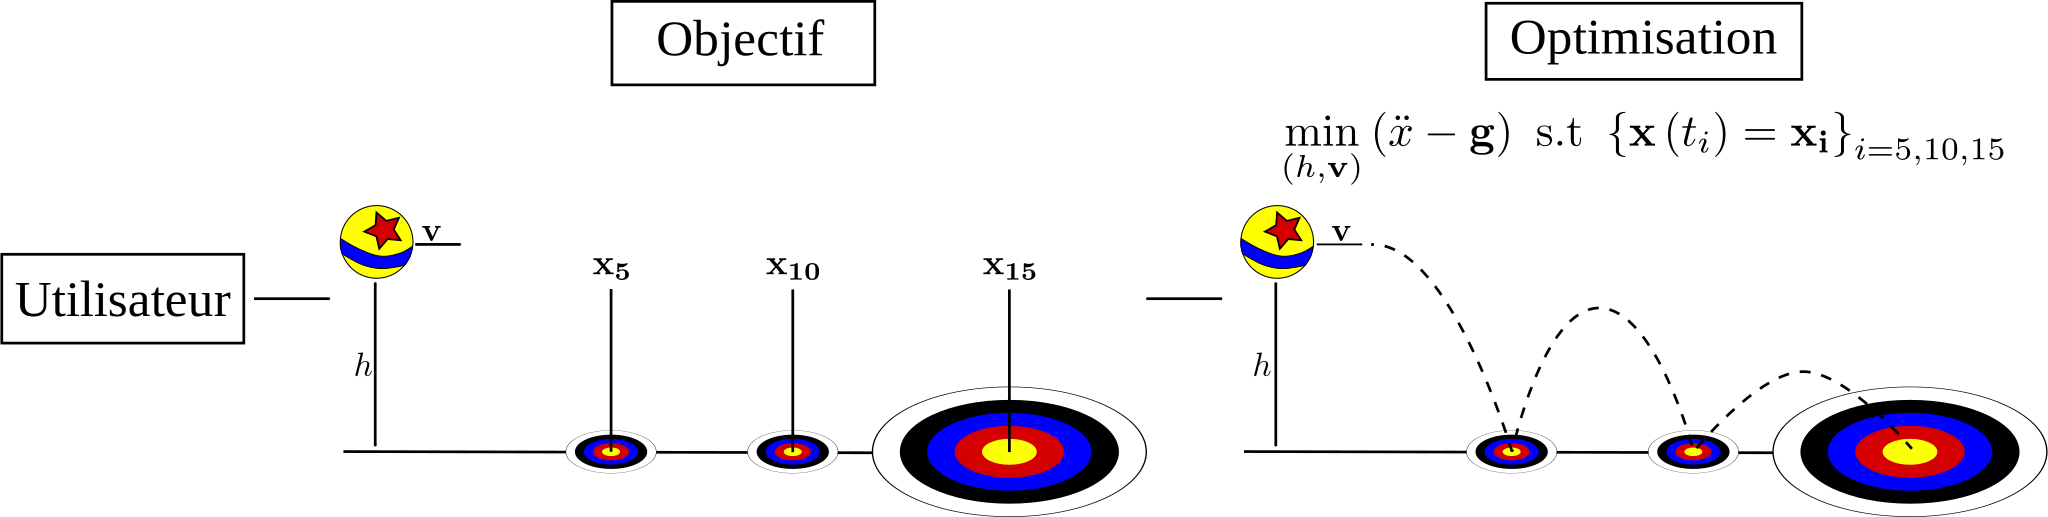
\includegraphics[scale=0.20]{./images/simulationControl/spaceTimeConstraints.png}
\caption[STAR control: Space-time constraints]{\label{fig:spaceTimeConstraints} Space-time constraints}
\end{figure}

\subsubsection{Parameters}
The most common parameters are the positions of the material samples and the \emph{wind} forces.
A common drawback of using \emph{wind} forces is that the necessary changes may become highly unrealistic for force due to wind. 
As an alternative, Coros et al.~\cite{Coros2012} proposed to adapt the rest shape of the object from one frame to another in order to induce internal forces that would match the user goals.
When large deformation occurs it is possible that the computed solution is at the limit of the deformation that the object can reach. In order to enforce the optimization, Li et al.~\cite{Li2014} proposed to optimize material parameters as well. 

\subsubsection{Constraints}
Position, velocity and density are among the constraints that are most often used for controlling an animation. 
Of course, they depend on the simulated object: rigid, solids, smoke, liquid, etc. 
Certainly, position constraints are the most intuitive for the user as they can be specified using key-frames. 
However, designing a key-frame for a highly elastic object or viscous materials might be extremely hard to achieve. 
Here there is a direct link to the works about surface modeling which propose to deform naturally an object \cite{Sorkine2007, Hildebrandt2011}. 
In some cases, these deformation tools can be seen as a local static simulation of the object that computes its deformation from a position change induced by the user. 
For elastic objects, such deformation tool has been proposed by Barbic et al.~\cite{Barbic2012}.
For liquids, Pan et al. \cite{Pan2013} propose an interactive method to deform wave shapes by sketching their profiles. 
Thus, direct spatial deformation is made possible. 
Both fits in the framework of surface modeling deformation. 
The only difference is that the function which are minimized are directly derived from the internal forces acting on the object. 
These methods are particularly useful when interactively editing an animation, specially when they are combined with high level deformation tools such as sketching.

\subsubsection{Numerical solution}
In their work, Witkin and Kass~\cite{Witkin1988} dealt with small systems and short simulation period.
Therefore, they could afford to directly solve the optimization problem, meaning that at each iteration a whole simulation would be computed. For instance, small rigid bodies simulation could be interactively designed through this approach \cite{Popovic2000},\cite{Popovic2003}. For complex models and large simulation time, this approach tends to take forever. Windowing methods allowed to restrict the optimization to the space-time range of interests \cite{Cohen1992}. In their work \cite{McNamara2004} proposed to use the adjoint method to efficiently compute gradients in liquid simulation thus improving the performance of the optimization. The approach was also used by Wojtan et al.~\cite{wojtan2006keyframe} for handling large particle systems. For elastic bodies, the use of reduced model allowed to achieve speed-ups of several order of magnitude, thus allowing to interactively edit a physics-based animation~\cite{Barbic2012},\cite{Hildebrandt2012}, \cite{Hahn2012}. Since, this approach has been further improved to be faster \cite{Schulz2014} and deal with large deformations \cite{Li2014}.

\subsection{Applications \& Alternatives}
The strength of the space-time constraints paradigm relies on its very general definition. Therefore, a large number of applications and methods can be seen as offsprings of this approach. In the following, we distinguished different applications of physics-based animation control and present alternatives to the above methods.

\subsubsection{Enriching an animation with physics}
Given a full animation, a simulation is run in order to enhance the input animation with detailed physically-based secondary motions. This approach was successfully applied to enhance character animation with wrinkles and folds of their skin by Bergou et al.~\cite{Bergou2007}. In their work, they compute the dynamics of thin shells on top of the animation by using a multi-resolution approach. In fluid animation, details enhancing brings a lot of attention as it would be easier to set up low resolution simulation and add details on top of it without loosing the global behavior. A nice approach was proposed by Mercier et al. \cite{Mercier2015} where they solve a Lagrangian wave simulation only at the surface of the low resolution simulation.

\subsubsection{Guiding a simulation with animation data}
A large number of methods propose to guide a simulation without the need of an expensive optimization problem. 
Generally these methods propose to use external forces that are automatically computed from the user inputs such as key-frames.
One of the first approach of this kind was proposed by Lamouret and Cani~\cite{Lamouret1996}.
This approach was later extended to more involved inputs such as simulation data.
In the case of fluid, user-defined velocity field~\cite{Kim2006:SmokeControl}, distance fields~\cite{Yang2013} and control particles~\cite{Thurey2006:FluidControl,Madill2013} were proposed to control the trajectory of fluid animation.
Still in the same idea, there are many methods which propose to guide the behavior of an object using geometric proxies which are easier to control for an artist than simulation data. For example, artists can use a triangle mesh to specify a target shape which will act as an attractor by adding artificial attraction forces based on the distance to the mesh surface. 
Such approaches have been successfully developed to drive smoke~\cite{Fattal2004,Hong2004,Shi2005a} and liquid simulations~\cite{Shi2005b,Raveendran2012}.
Taking this strategy further, the geometric proxies themselves can be defined by a low-resolution fluid simulation. 
To achieve this, the artist quickly sets up a coarse simulation and uses the output geometry to guide the main features of a full resolution simulation.
Several approaches modify a high-resolution smoke simulation using optimization~\cite{Nielsen2009,Nielsen2010}, patterns extracted as skeleton~\cite{Yuan2011}, or sparse sampling~\cite{Huang2013}.
For liquid simulations, Nielsen and Bridson~\cite{Nielsen2011} propose to restrict the high resolution simulation to a thin layer around a guiding coarse animation.
Although each of these approaches are able to successfully guide an animation, they do not enable direct control of the resulting animation. Designing precise timing or feature scaling would therefore still require iterative trial-and-error steps to converge toward a desired animation.

Alternatively, procedural tools enable faster editing loops.
Unfortunately, they are also based on indirect parameters setting and are often limited to overly restrictive fluid models such as large open ocean surfaces~\cite{hinsinger2002,Tessendorf2004,jeschke2015water,horvath2015empirical}.

\subsubsection{Example-based simulation}
Instead of controlling the trajectory of an object, one might want to control how it deforms when it collides with other objects. 
In exampled-based simulations, a set of examples that represent the desired deformations is used to build a space of preferred deformations from where internal forces will be deduced. This method was first introduced by Martin et al.~\cite{Martin2011} for elastic deformations. Jones et al.\cite{Jones2016} propose a similar method to easily incorporate plastic deformations in rigid bodies simulations.

\subsubsection{Animation sampling}
In multibody systems, the space-time constraints paradigm can hardly be used. In cause, the large number of discontinuous contacts events which makes the optimization problem particularly difficult to solve. In contrast, multibody simulators are particularly fast, so fast that it is possible to run in parallel a large number of simulations. In their work, \cite{Chenney2000} and \cite{Twigg2007} exploit this performance to sample the space of parameters of an animation and thus finding those which satisfy the user constraints.

\subsubsection{Animation editing} 
In contrast with simulation control, animation editing consists in deforming in space and time the output of a simulator without the need to re-simulate. 
Closely related to surface modeling it has to take into account the temporal dimension and its relation with space in order to propose new editing tools. 
In these approaches, finding a natural way to deform an animation and ensuring temporal consistency are amongst the main challenges.
Very few methods have been proposed whereas modifying the result of a simulation frame by frame is a common practice in animation studios. 
Among the most interesting approach, Pighin et al.\cite{Pighin2004} propose to build a space-time parametrization of a smoke animation using radial basis functions. 
Schpok et al.~\cite{Schpok2005} proposed to extract and parametrize features such as vortices, uniform advection, sinks, and sources to allow the user to modify the parameters in a smoke simulation.
For liquid animations, Raveendran et al.~\cite{Raveendran2014} match two liquids animations and propose a method to smoothly interpolate between them. 
This approach allows to quickly explore parameter space such as boundary conditions or viscosity parameter and then to produce a large number of new liquid animations without the need for re-simulation.

\subsection{Conclusion on simulation control}

All the above mentioned methods make a trade-off between realism and control.
On one hand, realism requires a high computational cost and makes methods such as space-time constraints unattractive for interactive use.
On the other hand, giving the user full control may introduce unphysical and unpleasant behavior.
Very few works explored the edit of an existing animation and how to extend classical modeling techniques to animated content.
We think that this approach would allow to interactively design physics-based animation without the need to re-simulate.
In Chapter~\ref{chap:fluidsculpting}, we will present a system for the design of fluid animation based on this idea.
\section{Conclusion}
There is a large number of techniques and models that are used to improve the efficiency of simulations, to simulate new phenomena and to allow the user to control a simulation.
We begin our contributions by extending an adaptive model, initially proposed for nanosystems simulations, to speed-up particle simulations in Computer Graphics, in Chapter~\ref{chap:arps}.
Then, we study how to perform detailed topological changes with the frame-based model in Chapter~\ref{chap:cutting}, an interesting approach which ensure a very small number of degrees of freedom and therefore interactive performances.
Finally, we explore a new way of editing fluid animations in Chapter~\ref{chap:fluidsculpting}, where the user can manipulate sub-part of the animation interactively without the need to re-simulate.



\cleartorecto

\include{chap3_starAdaptivity}

\cleartorecto

\chapter[Extending ARPS to Graphical Simulations]{Extending Adaptively Restrained Particle Simulation to Graphical Simulations}
\label{chap:arps}

\Lettrine{C}{ombining} efficiency with visual realism has been one of the main goals of computer graphics research in the last decade. 
In Chapter~\ref{chap:starAdaptivity}, we presented adaptive models, a general strategy to concentrate the computational time on the most interesting parts of an animated scene. 
We observed that the two main approaches consist of adapting time or spatial sampling. 
Although they can achieve impressive results, they are often difficult to implement, they may be restricted to specific applications and they sometimes generate discontinuity artifacts due to sudden simplifications.
\paragraph*{}
A different approach for adaptive simulation~\cite{Artemova2012} was proposed in the context of molecular dynamics~(MD). Contrary to most of the methods reviewed in Chapter~\ref{chap:starAdaptivity}, Adaptively Restrained Particle Simulations (ARPS) do not adapt time or spatial sampling, but rather switch the positional degrees of freedom of particles on and off, while letting their momenta evolve. The key idea is that since most of the computation time is spent in computing interaction forces based on positions, particles with low velocity could be considered fixed in space - and the corresponding interaction forces constant - until they accumulate enough momentum to start moving again. Therefore, inter-particles forces do not have to be updated at each time step, in contrast with traditional methods that spend a lot of time there.
\paragraph*{}
While freezing objects to gain computation time has been used in video games (see Section~\ref{sec:adaptive-integration}), the question of when and how to release them has not been extensively studied, and has mainly relied on \textit{ad hoc} heuristics.
Adaptively Restrained Particle Simulations~(ARPS), in contrast, introduce a physically sound approach with proven correctness, and has been successfully used in the context of predictive, energy-and momentum-conserving particle simulation.
\paragraph*{}
In this chapter, we explore the use of Adaptively Restrained (AR) particles for graphics simulations. Our experiments show that this new, simple strategy for adaptive simulations can provide significant speed-ups more easily than traditional adaptive models. The key contributions of our work are as follows: 
\begin{itemize}
\item We adapt ARPS to particle-based fluid simulations and propose an efficient incremental algorithm to update forces and scalar fields.
\item We introduce a new implicit integration scheme enabling to use ARPS for stiff objects simulations such as cloth.
\end{itemize}

The remainder of this chapter is organized as follows: 
Section~\ref{sec:arps_basics} presents the initial formulation of ARPS that was introduced for molecular dynamics simulations and explores its potential for computer graphics applications. 
Section~\ref{sec:arps_sph} and~\ref{sec:arps_implicit} respectively introduce our extension of ARPS to fluid and stiff objects simulations. 
Section~\ref{sec:arps_implementation} deals with the practical implementation and parameters tuning. 
Section~\ref{sec:arps_discussion} concludes and gives some perspectives of future works.
\paragraph*{}
The works described in this chapter were presented at the conference \emph{VRIPHYS 2013}~\cite{Manteaux2013}. 
A video illustrating the method and the results is available here: \url{https://youtu.be/RpJjGAoqp50}.
%-------------------------------------------------------------------------
\section{Adaptively Restrained Particles} 
\label{sec:arps_basics}
%-------------------------------------------------------------------------
\paragraph*{Basic ideas:}
Adaptively Restrained Particle Simulations (ARPS)~\cite{Artemova2012} were recently developed to speed up particle simulations in the field of Molecular Dynamics.
They rely on Hamiltonian mechanics, where the state of a particle system is described by a position vector $\vx$ and a momentum vector $\vp$, and its time evolution is governed by the following differential equations:
\begin{eqnarray*}
\frac{d\vp}{dt} &=& -\frac{\partial \H}{\partial \vx} \\
\frac{d\vx}{dt} &=& +\frac{\partial \H}{\partial \vp}
\end{eqnarray*}
Here, the Hamiltonian $\H$ is the total mechanical energy given by
\begin{equation}
    \label{eq:hamiltonian}
    \H(\vx,\vp) = \frac{1}{2} \vp^{T}M^{-1}\vp + V(\vx)
\end{equation}
where the first term corresponds to the kinetic energy, while the second represents the potential energy.
In~\cite{Artemova2012}, an \textit{adaptively restrained} (AR) Hamiltonian is introduced.
\begin{equation}
    \label{eq:arhamiltonian}
    \H_{AR}(\vx, \vp) = \frac{1}{2} \vp^{T}\Phi(\vx,\vp)\vp + V(\vx)
\end{equation}
The matrix $\Phi$ is a block-diagonal matrix used to switch on or off the positional degrees of freedom of the particles during the simulation.
Each $3$x$3$ block corresponds to a particle $i$ and is equal to
$\Phi_{i}(\vx_{i}, \vp_{i}) = m_{i}^{-1}[1 - \rho_{i}(\vx_{i}, \vp_{i})]\mathbf{I_{3\mathtt{x}3}}$.
The function $\rho_{i} \in [0, 1]$ is called the \emph{restraining function}.
When $\rho_{i} = 0$, $\Phi_{i} = m_{i}^{-1}$ and the particle is \textit{active}: it obeys standard (full) dynamics.
When $\rho_{i} = 1$, $\Phi_{i} = 0$ and the particle is \textit{inactive} (not moving). When $\rho_{i} \in [0, 1]$, the particle is in transition between the two states.
%-------------------------------------------------------------------------
The restraining function $\rho_{i}$ of each particle is used to decide \emph{when} to switch positional degrees of freedom on or off.
In~\cite{Artemova2012}, $\rho_{i}$ depends on the particle kinetic energy.
The function uses two thresholds, a restrained-dynamics threshold $\epsilon^{r}$ and a full-dynamics threshold $\epsilon^{f}$.
It is defined as
\begin{equation}
    \label{eq:restrainingfunction}
    \rho_{i}(\vp_{i}) =
    \displaystyle\left\lbrace
    \begin{array}{lccc}
        1, & & & \textrm{if } 0 \leq K_{i}(\vp_{i}) \leq \epsilon_{i}^{r} \\
        0, & & & \textrm{if } K_{i}(\vp_{i}) \geq \epsilon_{i}^{f} \\
        s(K_{i}(\vp_{i})) \in [0, 1], & & & \textrm{elsewhere} \\
    \end{array}
    \right.
\end{equation}
where $K_i=\vp_{i}^2/2m_{i}$ is the kinetic energy, and
$s$ is a twice-differentiable function. In practice a $5^{th}$-order spline is used.
%-------------------------------------------------------------------------
\paragraph*{Adaptive equations of motion:}
The adaptive equations of motions are derived from the AR Hamiltonian (Equation~\eqref{eq:arhamiltonian}).
\begin{equation}
   \label{eq:armotionequation}
    \displaystyle
    \begin{array}{l}
        \displaystyle \frac{d\vp}{dt} =
        -\frac{\partial \H_{AR}}{\partial \vx} = -\frac{\partial V(\vx)}{\partial \vx}\\ \\
        \displaystyle \frac{d\vx}{dt} =
       \frac{\partial \H_{AR}}{\partial \vp} = M^{-1}[I - \rho(\vp)] \vp
        - \frac{1}{2}\vp^{T}M^{-1}\frac{\partial \rho(\vp)}{\partial \vp}\vp\\
    \end{array}
\end{equation}
While the momenta evolve as in classical Hamiltonian mechanics, the positions evolve differently.
When a particle's momentum is small enough, the particle becomes inactive and stops moving.
However, even if the particle is inactive, its momentum may change.
Therefore its kinetic energy may become large enough again for the particle to resume moving.
In general, particles switch between active and inactive states during the simulation.
\paragraph*{}
Notice that $\displaystyle -\frac{\partial V(\mathbf{x})}{\partial \mathbf{x}}$ is equal to $\mathbf{f}(\mathbf{x})$, the forces applied on the particle system. In the initial formulation presented in Equation~\ref{eq:arhamiltonian}, these forces are conservative and only depend on positions. In Section~\ref{sec:arps_sph} and Section~\ref{sec:arps_implicit}, we detail how to use ARPS in dissipative systems where damping forces based on velocity are used.
\paragraph*{}
Finally, we introduce a notion that we will use in the following sections: the \textit{effective velocity}. It is the rate of position change of a particle $i$ and can be expressed by the following equation.
\begin{equation}
    \label{eq:adaptiveVelocity}
    \mathbf{v}_{i}^{eff} = \frac{1}{m_{i}} \left( (1-\rho_{i}(\vp_{i}))\vp_{i} - \frac{1}{2} \parallel \vp_{i} \parallel^2 \frac{\partial \rho_{i}(\vp_{i})}{\partial \vp_{i}}\right)
\end{equation}

\paragraph*{A simple example:}
Consider a 1D harmonic oscillator: a particle attached to the origin with a perfect spring.
Figure~\ref{fig:harmonicOscillatorPhasePortrait} shows a phase portrait of the corresponding
AR system.

\begin{figure}[!h]
	\centering
	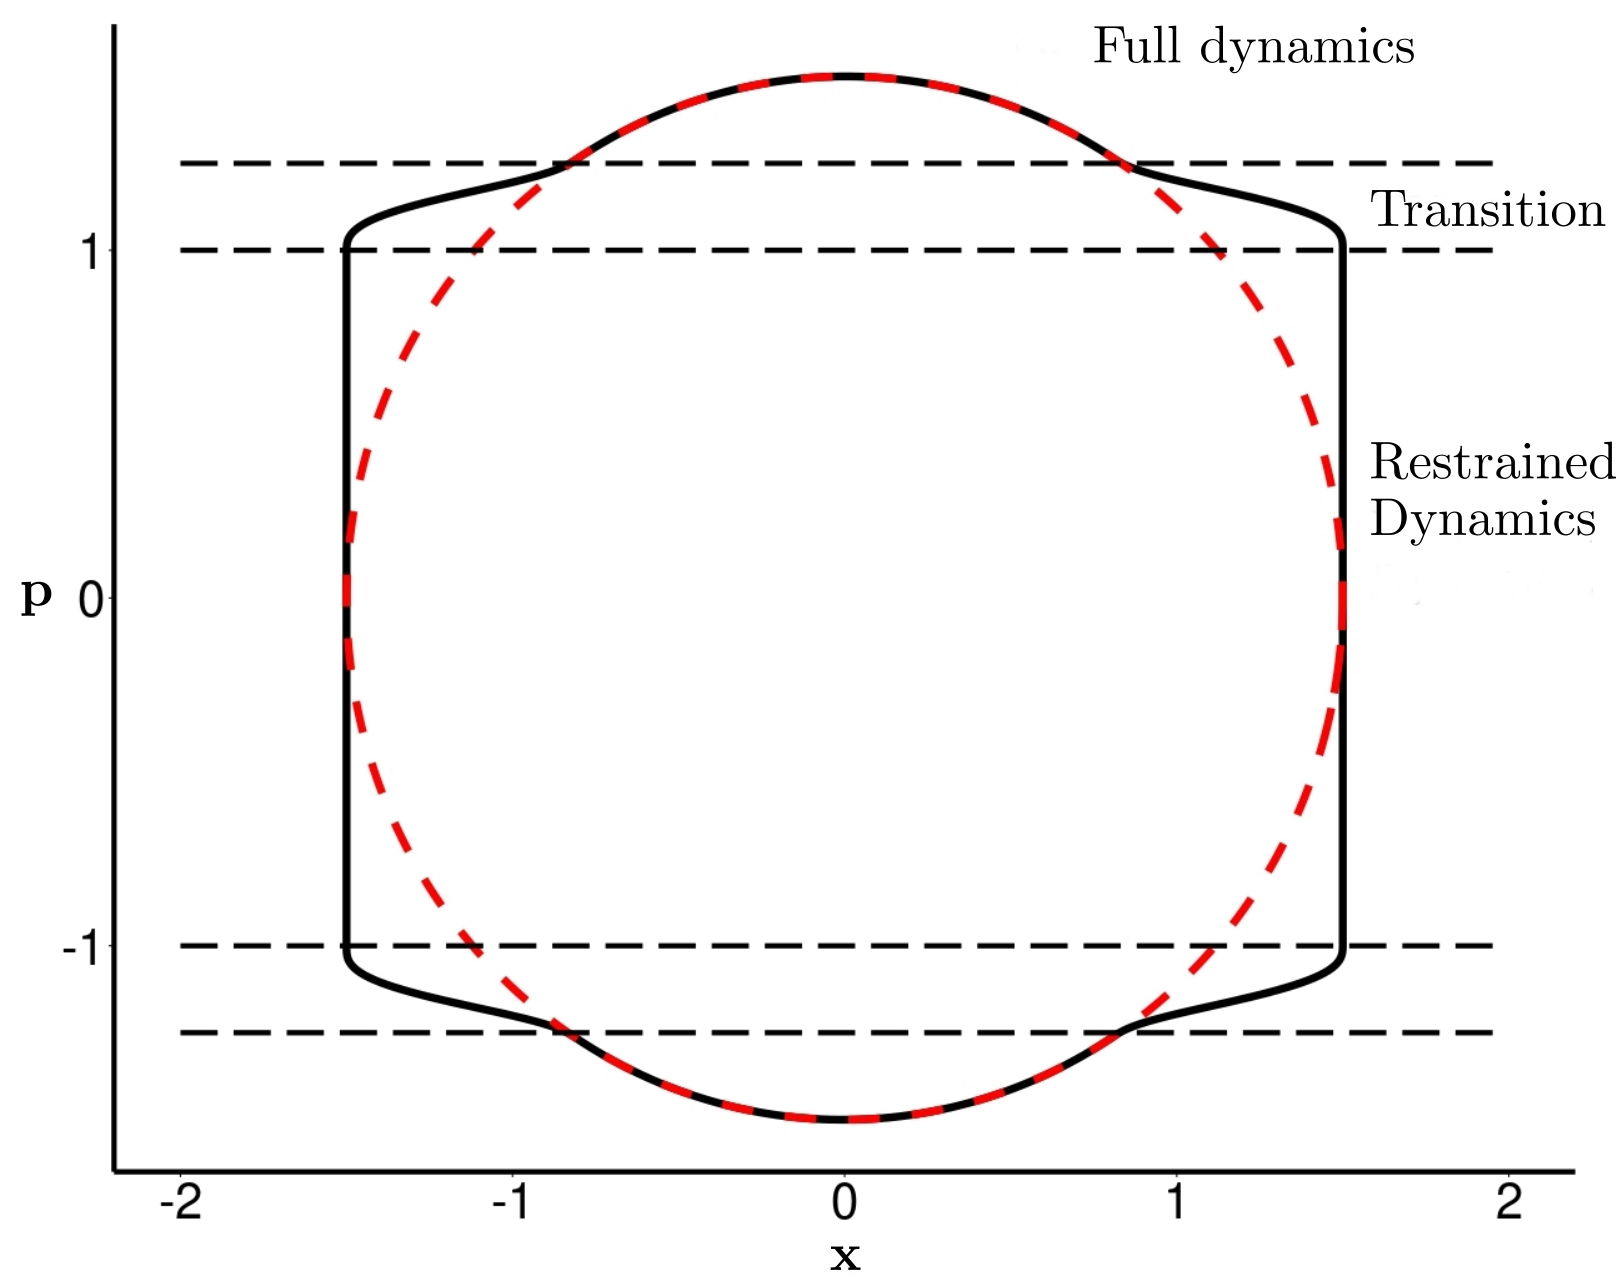
\includegraphics[width=0.8\linewidth]{images/arps-vriphys2013/harmonicOscillatorPhasePortraitraw_hacked.png}
	\caption[ARPS: Phase portrait of a ARPS harmonic oscillator]{\label{fig:harmonicOscillatorPhasePortrait} Phase portrait of a harmonic oscillator. The red dotted ellipse corresponds to standard Hamiltonian mechanics, while the solid black line corresponds to ARPS. During restrained dynamics, the particle's momentum is accumulated. When enough energy has been accumulated, a transition phase takes place leading the particle to switch back to full dynamics.}
\end{figure}

In classical mechanics, the trajectory of the state in this (position, momentum) space is an ellipse, the size of which depends on the (constant) energy of the system.
Using ARPS, the position is constant (vertical straight parts) as long as the kinetic energy is small enough, while it is an ellipse as long as the kinetic energy is large enough.
These trajectories are connected by a transition corresponding to an energy between the two thresholds of Equation~\eqref{eq:restrainingfunction}.
The closed trajectory corresponds to a constant \textit{adaptively restrained energy} $H_{AR}$.

\paragraph*{Generalization:}
Due to the similarity of the adaptive kinetic energy with the standard kinetic energy, particle systems simulated using ARPS exhibit the expected properties of standard physical simulation, namely the conservation of momentum and (adaptive) energy. It is therefore possible to perform macroscopically realistic simulations with reduced computation time as illustrated in Figure~\ref{fig:cascadeCollision}.

\begin{figure}[h!]
	\centering
	\includegraphics[width=1.0\linewidth]{images/arps-vriphys2013/ARPS_Collision_Artemova.png}
	\caption[ARPS: Collision Cascade from~\cite{Artemova2012}]{\label{fig:cascadeCollision} 
		A particle is launched at high velocity toward a 2D static particle system made of $5390$ particles, resulting into a collision cascade~\cite{Artemova2012}. 
		On the left, the result of a full dynamics simulation. 
		The three other images are the result of ARPS with different thresholds which allow a smooth trade between efficiency and precision.}
\end{figure}

%-------------------------------------------------------------------------
\paragraph*{Computational performance:}
The authors of~\cite{Artemova2012}, Artemova and Redon, obtained significant speed-ups by exploiting the immobility of particles. Figure~\ref{fig:cascadeCollision} illustrates one of their result where a $10\times$ speed-up was achieved in a collision scenario while keeping a behavior close to the reference one. In this example, inter-particles forces were derived from a Lennard-Jones potential. To save time on inactive particles, they proposed an incremental method to update the particles' forces at each time step:
\begin{enumerate}
    \item All forces that were acting on each active particle at the previous time step are subtracted based on previous position.
    \item New forces based on current positions are added to each active particle.
\end{enumerate}
The increase of computational performance comes from the absence of force computation between
two inactive particles and the absence of neighbor search for inactive particles.
As these two steps are common bottlenecks in particle simulation, significant speed-up can be achieved.

%-------------------------------------------------------------------------
\paragraph*{Potential benefits of extension to computer graphics:}
Molecular dynamics often inspired particle-based simulations in computer graphics. The same bottleneck, namely inter-particles forces computation based on neighbor search, is present in the two fields, so we can expect interesting performance for ARPS in graphics. The remainder of this chapter explores two applications of ARPS to graphical simulations:
\begin{enumerate}
\item Particle-based fluid simulation. Originally, ARPS has been applied to conservative system. While fluid simulation involves position-based forces, it also involves velocity-based viscosity forces that need to be taken care of. We propose a simple method to handle them. Additionally, we extend the incremental algorithm proposed by Artemova and Redon to update forces as well as scalar fields.
\item Stiff object simulation. Explicit integration of stiff objects such as cloth is expensive due to stability issues. A well known solution is to use implicit integration instead. We derive an implicit formulation of ARPS and propose a hybrid solver to exploit the inactivity of particles in cloth simulation.
\end{enumerate}
It is clear that ARPS is not well-suited for simulations where all degree of freedom move: classical spatial adaptation is better suited in this case. In contrast, ARPS is best suited for simulations where most parts are immobile but may resume moving at any time. Even if these situations are not the most visually exciting, they are very common in computer graphics: they include simulation of characters clothing when many of the characters are at rest, surgical simulations with local-only user interaction, and the animation of large volumes of liquid, when most of it already came to rest.

%-------------------------------------------------------------------------
\section{ Extension to SPH fluid simulation } 
\label{sec:arps_sph}
As presented in section~\ref{subsubsec:starSPH}, SPH fluid simulation is widely used in computer graphics and many methods have been proposed~\cite{Desbrun1996},~\cite{Muller2003},~\cite{Solenthaler2009},~\cite{Ihmsen2014:IISPH}.
SPH approximates fluid dynamics with a set of particles.
The particles are used to interpolate the properties of the fluid anywhere in space.
Each particle samples the fluid properties such as density, pressure or temperature. All these properties are updated based on the particle neighbors and are
used in short-ranged inter-particle forces.
\subsection{ Incremental update }
To integrate ARPS, we chose WCSPH (Weakly Compressible Smoothed Particle Simulation)~\cite{Becker2007WCSPH}, a standard SPH formulation~\cite{Desbrun1996},~\cite{Muller2003}. For the sake of simplicity, we limit our discussion to the main inter-particles forces: pressure and viscosity. 
Algorithm~\ref{alg:WCSPH} describes the classical simulation loop.

\newpage

\begin{algorithm}[H]
    \caption[ARPS: WCSPH simulation]{WCSPH simulation loop}
    \label{alg:WCSPH}
    \begin{algorithmic}
	\ForAll{particle $i$}
	    \State find neighbors $j$
    \EndFor
    \ForAll{particle $i$}
    \State compute density $\rho_{i}$ (e.g. Eq.~\ref{eq:densitySPH})
    \State compute pressure $p_{i}$ using $\rho_{i}$ (e.g. Eq.~\ref{eq:pressureSPH})
    \EndFor
    \ForAll{particle $i$}
    \State $\displaystyle \mathbf{f}_{i}^{pressure} = -\frac{m_{i}}{\rho_{i}}\nabla p_{i}$ (e.g. Eq.~\ref{eq:pressureGradientSPH})
    \State $\displaystyle \mathbf{f}_{i}^{viscosity} = m_{i}\eta\nabla^{2}\mathbf{v}_{i}$ (e.g. Eq.~\ref{eq:velocityLaplacianSPH})
    \State $\displaystyle \mathbf{f}_{i}(t) = \mathbf{f}_{i}^{pressure} + \mathbf{f}_{i}^{viscosity} + \mathbf{f}_{i}^{other}$
    \EndFor
    \ForAll{particle $i$}
    \State $\mathbf{v}_{i}(t+\Delta t) = \mathbf{v}_{i}(t) + \Delta t \mathbf{f}_{i}(t)/m_{i}$
    \State $\mathbf{x}_{i}(t+\Delta t) = \mathbf{x}_{i}(t) + \Delta t \mathbf{v}_{i}(t+\Delta t)$
    \EndFor
    \end{algorithmic}
\end{algorithm}

ARPS can save time on each computation step involving the position of the particles.
In SPH fluid simulation, every property of a particle is computed as a weighted sum of its neighbors' property.
And the weights are computed based on the position of the particle and its neighbors.
Therefore, time can be saved as soon as a particle is close to immobility. 
This makes SPH a perfect candidate for ARPS.
\paragraph*{}
As long as a particle is inactive and is surrounded by inactive particles, its properties and neighborhood do not need to be updated.
In practice, this includes pressure and viscosity forces as well as density and pressure scalar field.
\paragraph*{}
To gain computational time from the inactive particles, we extend the incremental algorithm proposed in~\cite{Artemova2012} (see Algorithm~\ref{alg:WCSPHARPS}).
In this algorithm we denote as \emph{active} every \emph{active} or {transitive} particle.
From one step to another, only the contributions to physical properties from active particles are updated. 
Thus, even inactive particles whose neighbors are active are kept up-to-date.

\newpage

\begin{algorithm}[H]
    \caption[ARPS: WCSPH+ARPS simulation]{WCSPH+ARPS simulation loop}
    \label{alg:WCSPHARPS}
    \begin{algorithmic}
        \If{step=1}
        \State Perform Algorithm~\ref{alg:WCSPH}
        \Else
            \ForAll{\textbf{active} particle and its neighbors $i$}
            \State Subtract old density contribution from neighbor $j$
	        \State Subtract old pressure/viscosity force contribution from neighbor $j$
            \EndFor
            \ForAll{\textbf{active} particle neighbors $i$}
            \State find neighbors $j$
            \EndFor
            \ForAll{\textbf{active} particle and its neighbors $i$}
            \State Add new density contribution from neighbor $j$
            \State Update pressure $p_{i}$
	        \State Add new pressure/viscosity force contribution from neighbor $j$
            \State Add new density contribution from neighbor $j$
            \EndFor
            \ForAll{particle $i$}
            \State $\mathbf{v}_{i}(t+\Delta t) = \mathbf{v}_{i}(t) + \Delta t \mathbf{f}_{i}(t)/m_{i}$
            \State $\mathbf{x}_{i}(t+\Delta t) = \mathbf{x}_{i}(t) + \Delta t \mathbf{v}^{eff}_{i}(t+\Delta t)$
            \State Update particle's state based on $\rho(\mathbf{p_{i}})$.
            \EndFor
        \EndIf
    \end{algorithmic}
\end{algorithm}

\newpage 

%-------------------------------------------------------------------------------
\subsection{Viscosity}
In SPH, viscosity forces play an important role in the stability of the simulation and in the range of phenomena that can be simulated. 
However, ARPS was designed for conservative systems and no damping terms involving the velocity of the particle is involved, as we can see in the equation of motion (see Equation~\ref{eq:armotionequation}).
In ARPS, velocity can be represented in two different ways.
We may define it based on the momentum and set $\mathbf{v}_{i} = \vp_{i} / m_{i} $, or based on the \emph{effective velocity} $\mathbf{v}_{i}^{eff}$ defined in Equation~\ref{eq:adaptiveVelocity}.
In the first case, we can get time-varying forces even for inactive particles, which we want to avoid.
We therefore use the effective velocity of the particle, as defined in Equation(\ref{eq:adaptiveVelocity}).
Applied to a harmonic oscillator, this results in the behavior illustrated in Figure:\ref{fig:HODampedPP}.
The more the particle is damped the longer it remains inactive, which is an intuitive behavior.
%%% HARMONIC OSCILLATOR DAMPED%%%
\begin{figure}[H]
  \centering
  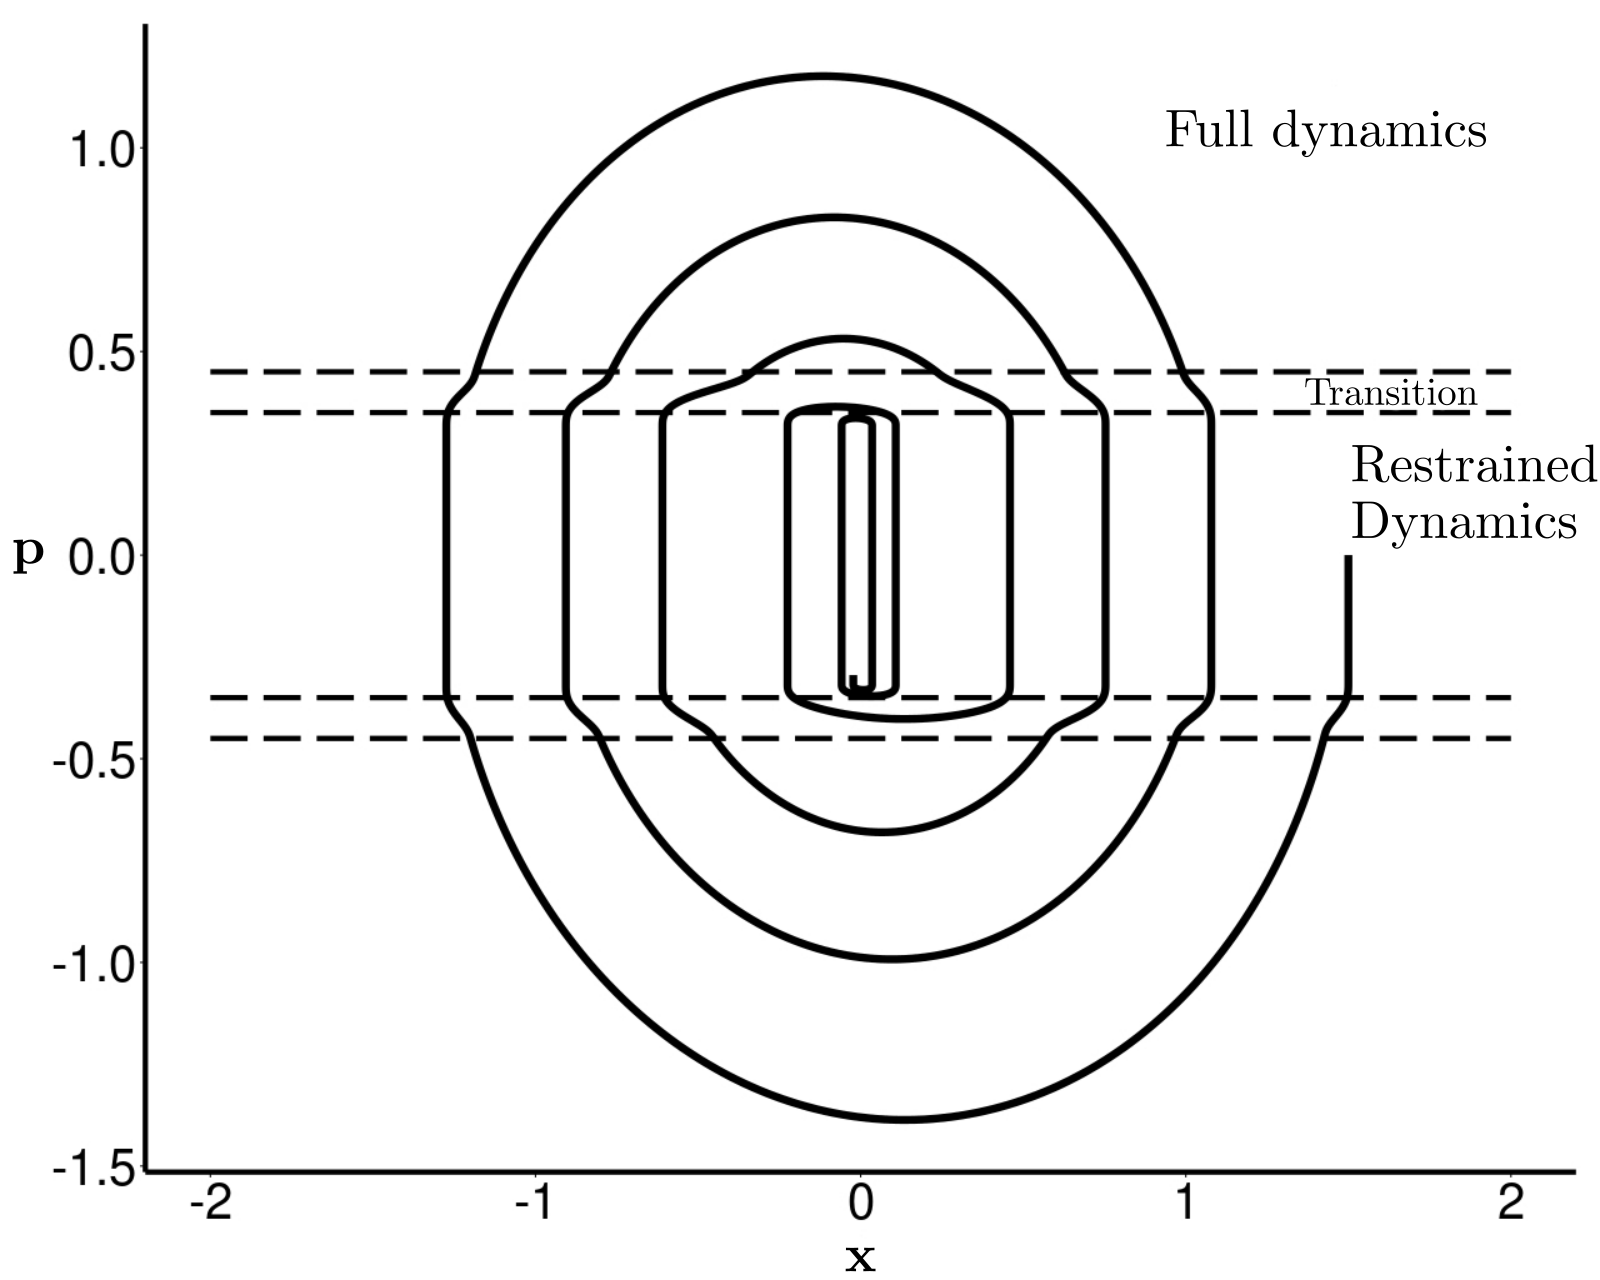
\includegraphics[width=0.8\linewidth]{images/arps-vriphys2013/harmonicOscillatorDampedPhasePortraitraw_hacked.png}
  \caption[ARPS: Phase portrait of a damped ARPS harmonic oscillator]
  {\label{fig:HODampedPP} Phase portrait of our viscosity approach in ARPS.
  As with a classic damped oscillator we obtain a spiral phase portrait.}
\end{figure}
%-------------------------------------------------------------------------
\subsection{Modified inactivity criterion}
Since our viscosity force vanishes along with the effective velocity of the particle, it drags down the kinetic energy asymptotically close to the inactivity threshold, without ever reaching it.
Consequently, particles only subject to viscosity forces never become inactive, and we do not spare computation time, even when the particles get nearly static.
To remedy this problem, we consider inactive the particles which effective velocity fall below a user-defined threshold.

%-------------------------------------------------------------------------
\subsection{Performance}
We performed two experiments to measure computation time.
The first one is a classical dam break simulation made of $5000$ particles.
We can see in Figure~\ref{fig:ARPS_Teaser} that during fast movements most of the particles are active and the adaptive simulation stays close to reference simulation.
Therefore small scale details like splashes are preserved.

\begin{figure}[!h]
	\begin{tabular}{cc}
		\includegraphics[width=0.4\linewidth]{images/arps-vriphys2013/ReposSPHClassique1.jpg} &
		\includegraphics[width=0.4\linewidth]{images/arps-vriphys2013/ReposSPHARPSColor1.jpg}
	\end{tabular}
	\centering
	\caption[ARPS: Dam break simulations]{ A dam break simulation with 5000 particles simulated with WCSPH (on the left)
		and with our adaptive method (on the right). On the right image, blue corresponds to full-dynamics particles, green to transition particles and red to restrained particles.}
	\label{fig:ARPS_Teaser}
\end{figure}

As soon as most particles come to rest and become inactive the speed-up can be significant (see Table~\ref{table:perf1}).
For $15$s, the mean speed-up is $3.8$.
The speed-up can locally reach $25.7$.

\begin{table}[h!]
	\centering
	\begin{tabular}{|c|c|c|c|} \hline
		Simulation Time & SPH   & ARPS    & Speed-up \\ \hline
		15s     & 893s   & 232s                 &  \{0.91, 25.73, 3.85\}\\ \hline
	\end{tabular}
	\caption[ARPS: Dam break - Measurements]{\label{table:perf1}Dam break - Computation time and speed-up \small{\{min, max, mean\}}}
\end{table}

The second experiment is the creation of a permanent flow with $4240$ particles. As we can see in Figure~\ref{fig:permanentflow}, once the permanent flow is installed a large amount of particles are restrained. 
We reach an interesting speed-up while keeping a motion close to the reference (see Table~\ref{table:perf2}).

\begin{table}[h!]
	\centering
	\begin{tabular}{|c|c|c|c|} \hline
		Simulation Time & SPH       & ARPS    & Speed-up \\ \hline
		30s         & 2166s     & 814s              & \{0.83, 3.99, 2.66\} \\ \hline
	\end{tabular}
	\caption[ARPS: Permanent flow - Measurements]{\label{table:perf2}Permanent flow - Computation time and speed-up \small{\{min, max, mean\}}.}
\end{table}

\newpage 

\begin{figure}[!h]
	\centering
	\begin{tabular}{ccc}
		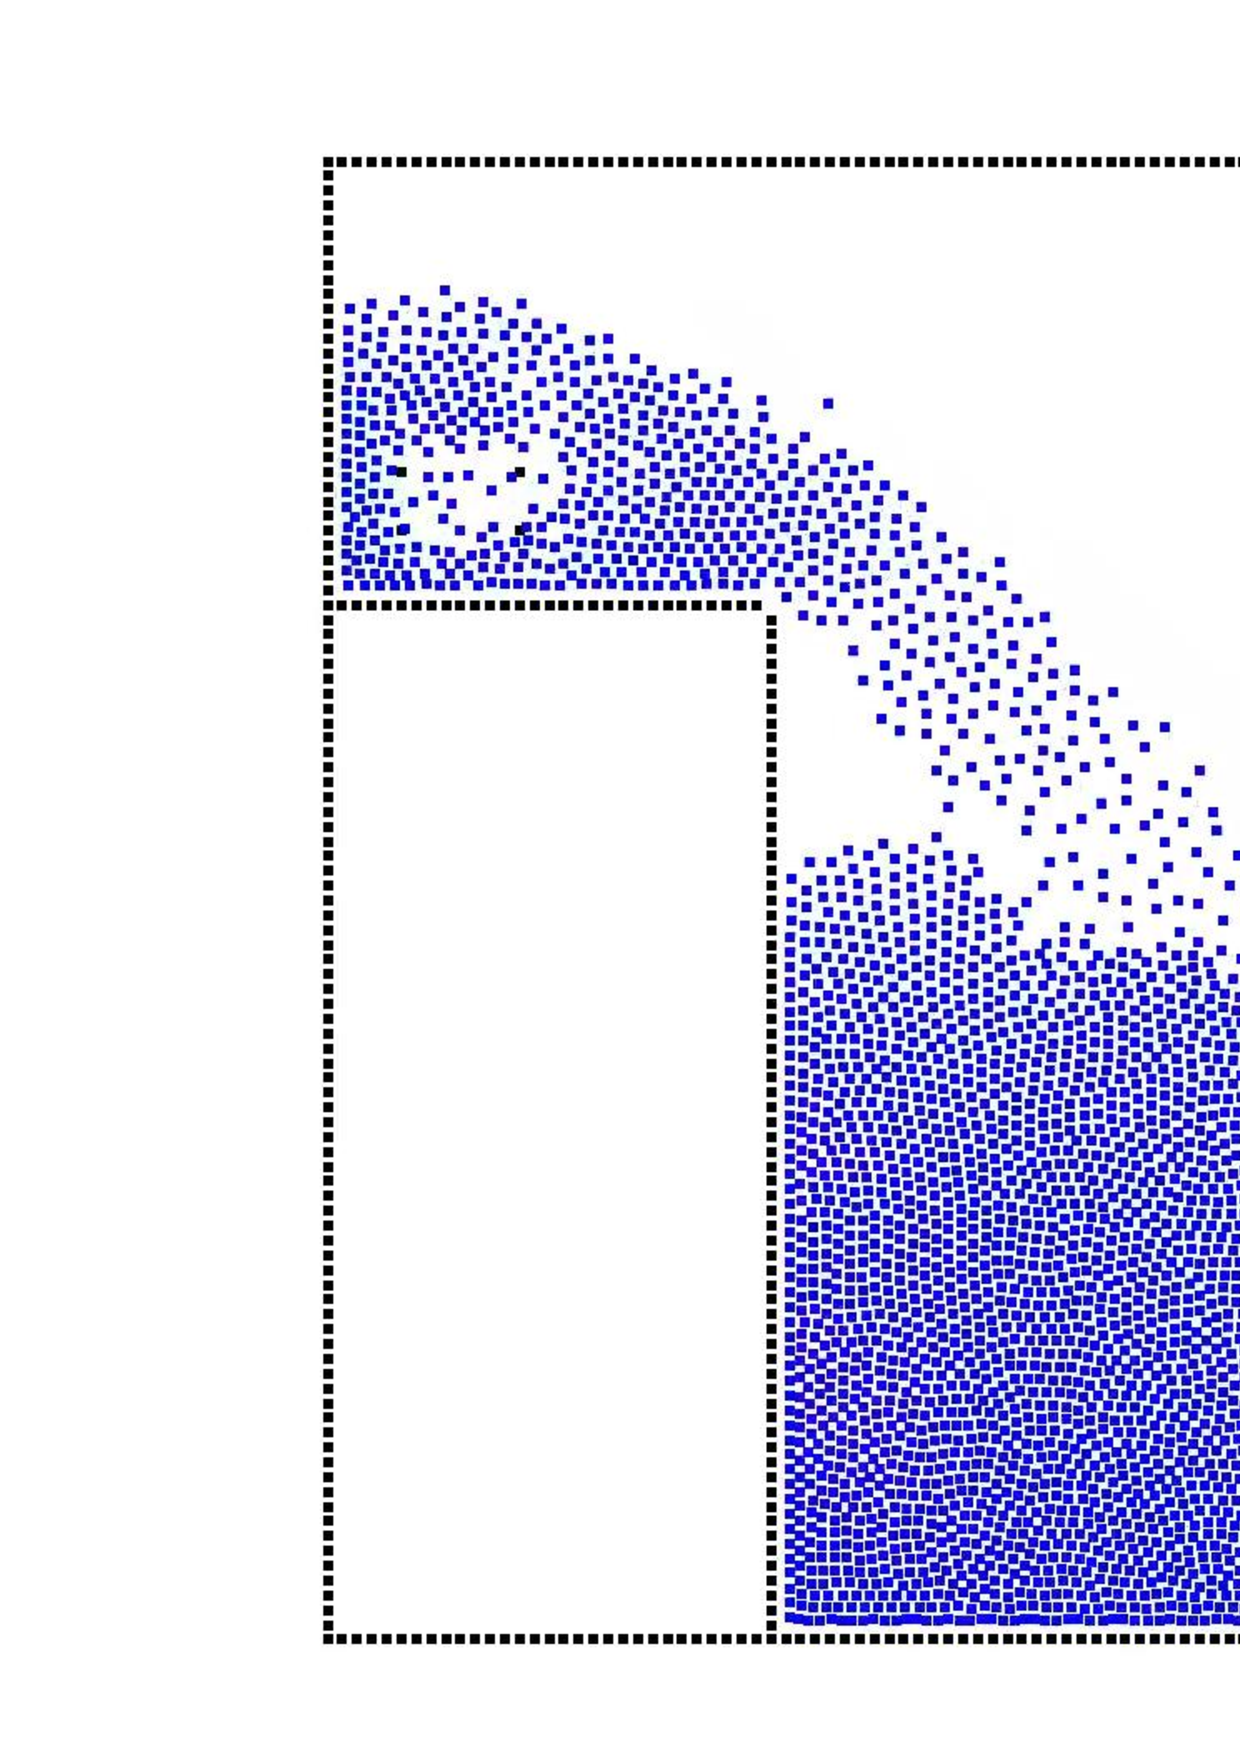
\includegraphics[width=.32\linewidth]{images/arps-vriphys2013/PermanentFlowSPH.jpg} &
		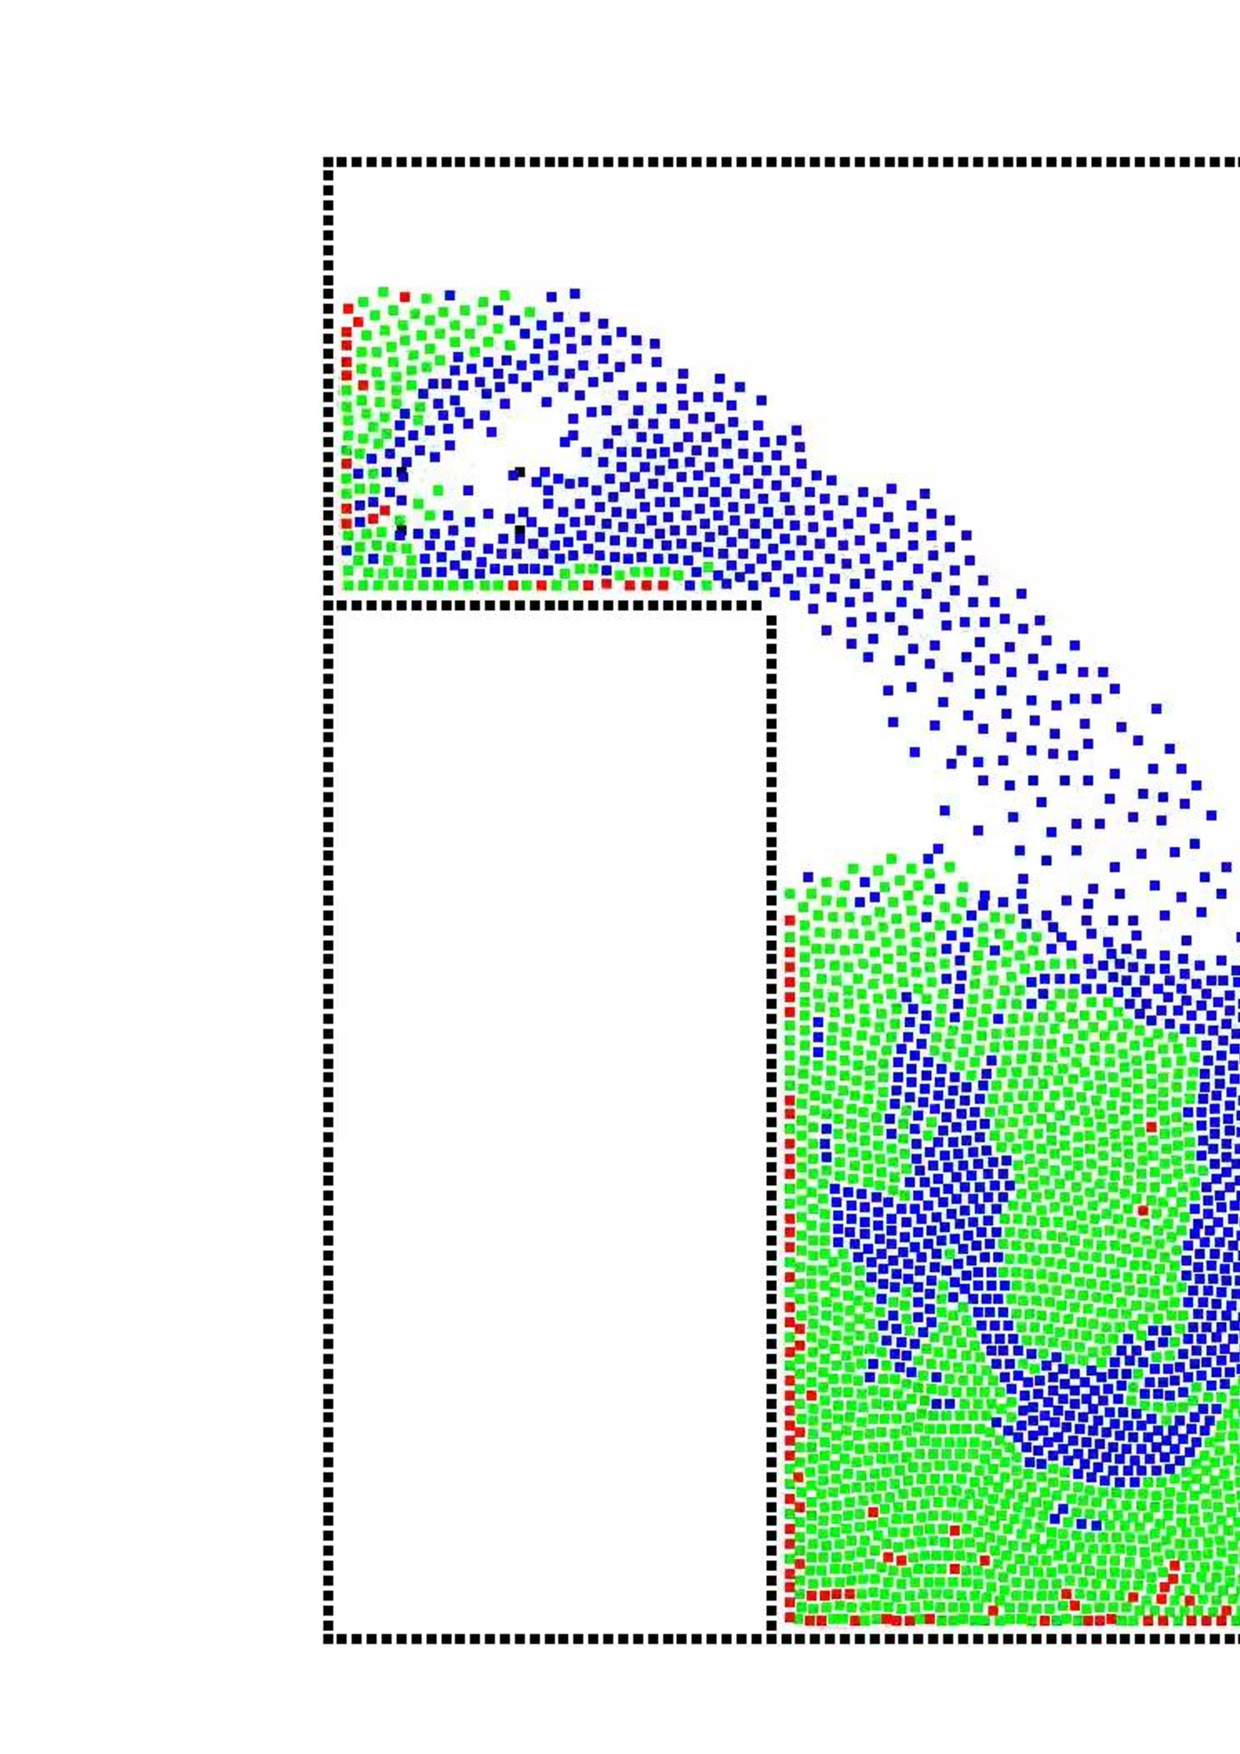
\includegraphics[width=.32\linewidth]{images/arps-vriphys2013/PermanentFlowARPSColor.jpg} &
		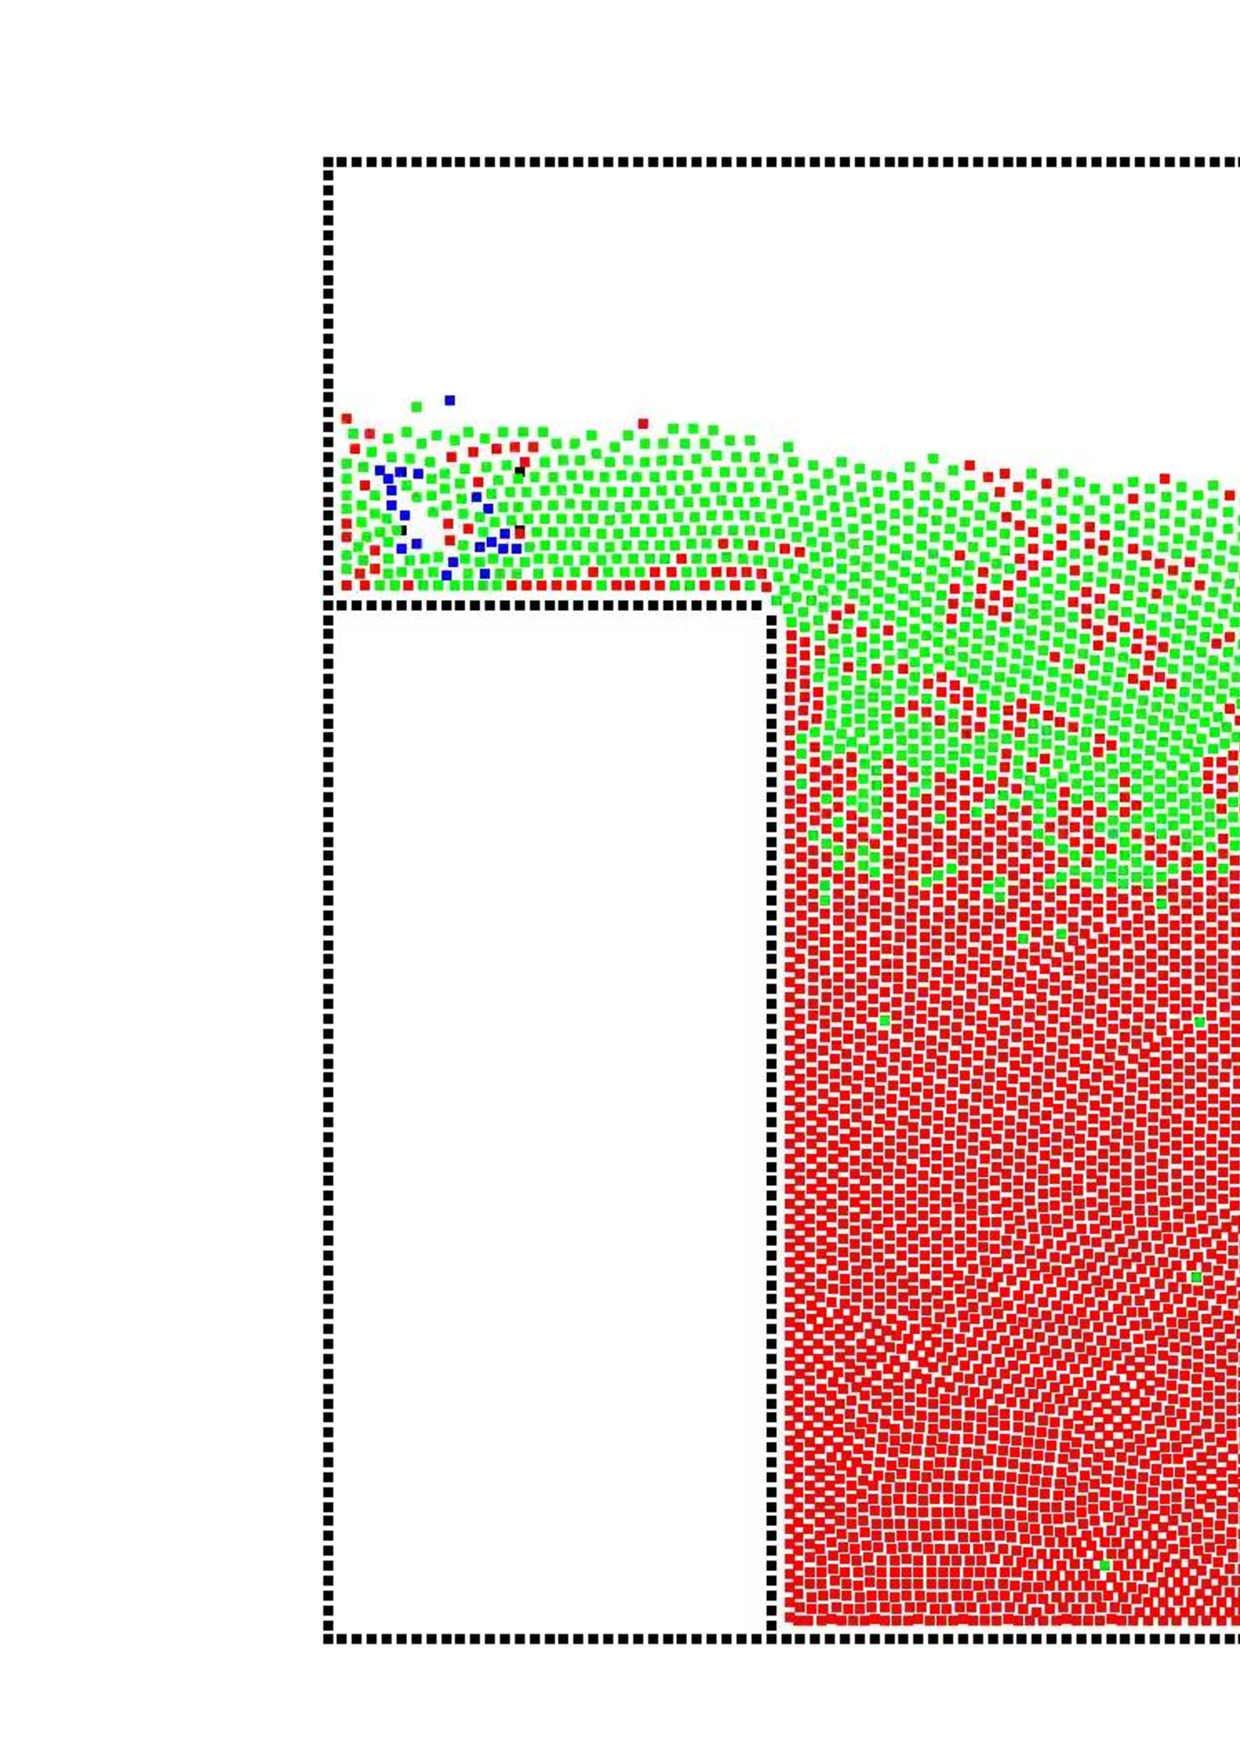
\includegraphics[width=.32\linewidth]{images/arps-vriphys2013/PermanentFlowARPSColor2.jpg} \\
		(a) & (b) & (c)
	\end{tabular}
	\caption[ARPS: Permanent flow simulations]{\label{fig:permanentflow} A permanent flow simulation with 4240 particles.
		(a) is a classic WCSPH simulation. (b) is our adaptive method at the same time step as (a) with restrained particles in red. (c) is our adaptive method once the permanent flow is installed.}
\end{figure}

These examples show that ARPS can effectively be extended to speed up liquid simulation in computer graphics. The next section consider its application to cloth animation.

%-------------------------------------------------------------------------
\section{Extension to stiff objects: Implicit Integration} 
\label{sec:arps_implicit}
In this section we explore the application of ARPS to stiff objects simulations, such as clothes, and propose an implicit integration scheme which saves computation time for particles at rest.
Implicit integration for cloth simulation was introduced by Baraff~and~Witking~\cite{Baraff1998}. 
An introduction to implicit integration is proposed by Witkin et al.~\cite{Witkin2001}.
While originally formulated on velocity, it can be straightforwardly expressed on momentum.
Instead of integrating the momentum using the forces at the current time step, implicit integration uses the forces at the end of the current step.
As we do not know these forces we end up with a non linear function.
We can linearize this function and solve the resulting linear system to obtain the next momentum
\begin{equation}
    \label{eq:implicit}
    ( I -\Delta t^{2}KM^{-1} ) \Delta \vp = \Delta t( \vf + \Delta t KM^{-1}\vp ) \;,
\end{equation}
where $\mathbf{f}$ are the forces applied on the system, $\displaystyle K = \frac{\partial \vf}{ \partial \vx}$ is the stiffness matrix and $M$ is the mass matrix. 
Solving the linear system is more costly than explicit integration, but it allows the use of larger time steps without any loss of stability, enabling to advance much faster.
For our experiments, we used simple spring forces between particles.
%------------------------------------------------------------------------
\subsection{ ARPS Implicit Integration }
We derive an implicit integration scheme from Adaptively Restrained equations of motion.
The linear system has to take into account the state of the particles.
The discrete equations of motions for implicit Euler are
\begin{equation}
	\label{eq:implicitEqMotion}
	\begin{array}{l}
	\displaystyle \Delta \vp =  \Delta t \vf(\vx_{n+1}, \vp_{n+1})\\
				\\
	\displaystyle \Delta \vx = \Delta t \left( M^{-1}(1-\rho(\vp_{n+1}))\vp_{n+1} \right. \\
	\displaystyle \left. - \frac{1}{2}\vp_{n+1}^{T} M^{-1} \frac{\partial \rho(\vp_{n+1})}{\partial \vp}\vp_{n+1} \right)
	\end{array}
    .
\end{equation}
We perform a Taylor-Young expansion of $\vf(\vx_{n+1}, \vp_{n+1})$ and introduce $\Delta \vx$ in the expended momenta equation.
We then perform a Taylor-Young expansion of $\rho(\vp_{n+1})$ in the momentum equation, which gives us the following equation system.
\begin{equation}
	\label{eq:arpsLinearSystem}
	( I -\Delta t^{2}KRM^{-1} ) \Delta \vp = \Delta t( \vf + \Delta t KM^{-1}s )
\end{equation}
$R$ is a block-diagonal matrix where each $3\times 3$ block $R_{ii}$ is
\begin{equation}
	\label{eq:Ri}
	\begin{array}{l}
	\displaystyle R_{ii} = I - \rho(\vp^{i}_{n}) - \vp^{i}_{n} \frac{\partial \rho(\vp^{i}_{n})}{\partial \vp_{i}}^{T} \\
	\displaystyle - \frac{1}{2}\vp^{i}_{n}\vp^{i^{T}}_{n}\frac{\partial^{2} \rho(\vp^{i}_{n})}{\partial \vp_{i}^{2}}^{T} -
	\displaystyle \frac{\partial \rho(\vp^{i}_{n})}{\partial \vp_{i}} \vp^{i^{T}}_{n} \;,
	\end{array}
\end{equation}
while $s$ is a $3N$ vector where $N$ is the number of particles, and each $s_{i}$ is
\begin{equation}
	\label{eq:si}
	\displaystyle s_{i} = \vp^{i}_{n} - \rho(\vp^{i}_{n})\vp^{i}_{n} - \frac{1}{2	}\vp^{i^{T}}_{n}\vp^{i}_{n}\frac{\partial \rho(\vp^{i}_{n})}{\partial \vp_{i}}.
\end{equation}
Note that if all particles are inactive then we have $R = 0$ and $s = 0$ and we get an explicit formulation.
\begin{equation}
    \label{eq:ARPSImplicitRestrained}
    I \Delta \vp = \Delta t \vf
\end{equation}
Conversely, if all particles are active then $R = I$ and $s = \vp$ and we get the classical implicit formulation of Equation(\ref{eq:implicit}).
In the general case, we loop over time using algorithm~\ref{alg:ARPSimplicit}.
\begin{algorithm}[H]
    \caption[ARPS: Implicit integration scheme]{Implicit integration scheme}
    \label{alg:ARPSimplicit}
    \begin{algorithmic}[10]
	\For{ each time step}
	    \State compute $\rho, R, s, \vf$.
	    \State compute $A = I - \Delta t^{2}KRM^{-1}$
	    \State compute $b = \Delta t \vf + \Delta t^{2}KM^{-1}s$
	    \State solve $A \Delta \vp = b$
            \State compute $\vp_{n+1} = \vp_{n} + \Delta \vp$
	    \State compute $\displaystyle \vx_{n+1} = \vx_{n} +
            \Delta t M^{-1}\left( R\Delta \vp+ s \right)$
	\EndFor
    \end{algorithmic}
\end{algorithm}

Figure~\ref{fig:implicitHOPP} shows the phase portrait of a harmonic oscillator simulated using our implicit formulation.
As expected, the well-known numerical damping effect of implicit Euler provides us with the same behavior we could observe with a damped harmonic oscillator.

%%% IMPLICIT HARMONIC OSCILLATOR DAMPED%%%
\begin{figure}[!h]
	\centering
	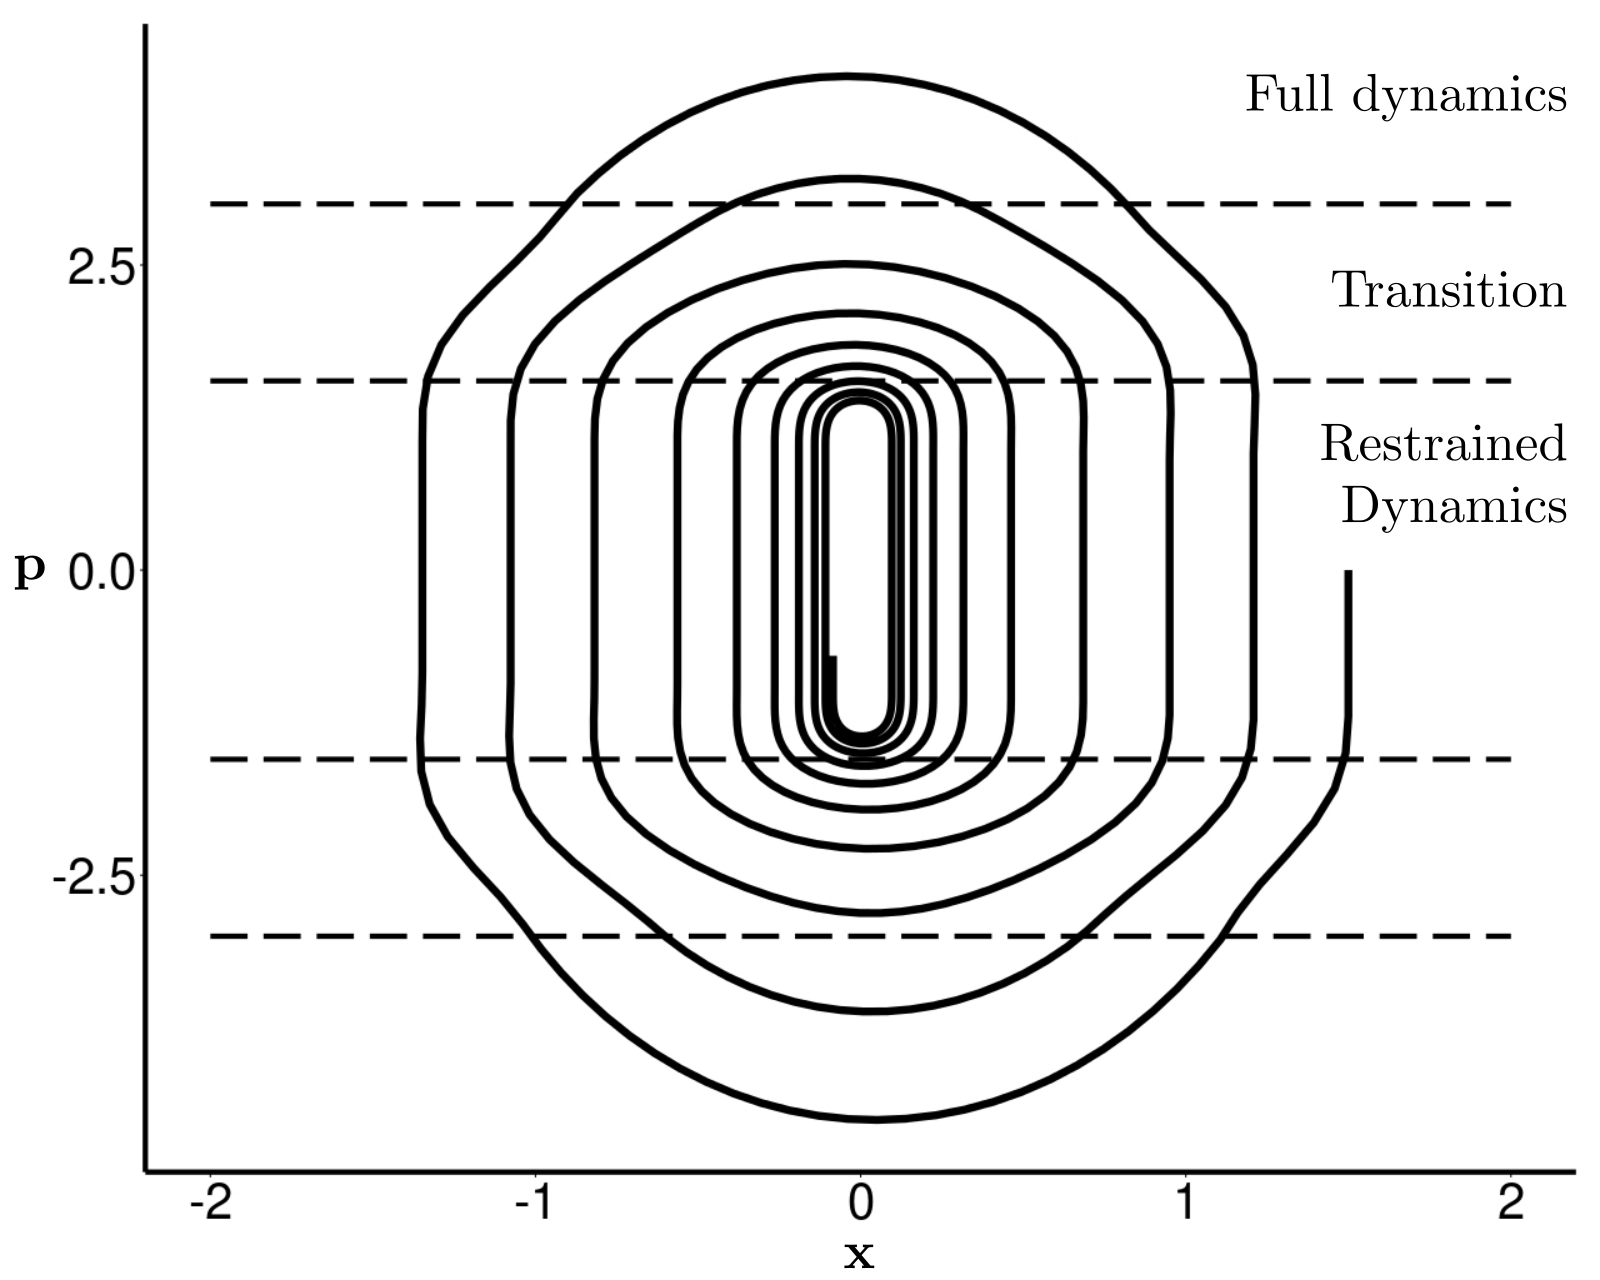
\includegraphics[width=0.8\linewidth]{images/arps-vriphys2013/implicitHOPPraw_hacked.png}
	\caption[ARPS: Phase portrait of an implicit ARPS harmonic oscillator]{\label{fig:implicitHOPP} Phase portrait of an implicit ARPS harmonic oscillator.}
\end{figure}

To include a more controllable damping term in the physical model, we derived an implicit formulation which includes a damping term $\vf_{d} = -\gamma \mathbf{v}^{eff}$.
\begin{equation}
	\label{eq:arpsLinearSystemDamped}
	( I + \Delta t \gamma M^{-1}R -\Delta t^{2}KRM^{-1} ) \Delta \vp = \Delta t( \vf + \Delta t KM^{-1}s + \vf_{d})
\end{equation}

%------------------------------------------------------------------------
\paragraph*{Solving the equation:}
We exploit inactive particles to save computation time.
As discussed earlier, inactive particles can be handled using explicit integration, which is much simpler.
When a particle is inactive and has no active neighbors we do not need to include it in the linear system.
We thus build the minimal linear system, which only contains active particles and their neighbors.
These particles are implicitly integrated, while the others are explicitly integrated.
\paragraph*{}
Figure~\ref{fig:clothARPS} shows a hanging cloth with active and inactive particles.
At the beginning all the particles become active. Then a moving front of inactivation/reactivation traverses the cloth at decreasing frequency. The cloth finally finds a rest position, where all the particles are inactive and simulated explicitly, saving computation time. The particles can become active again if external forces or imposed motion are applied.
Table~\ref{tab:clothePerf} shows performances we achieved with our hybrid solver.
As soon as a large number of particles become inactive the simulation is explicitly integrated and interesting speed-up can raise.

\begin{figure}[!h]
	\centering
	\includegraphics[width=0.8\linewidth]{images/arps-vriphys2013/Square3.jpg}
	\caption[ARPS: ARPS cloth simulation]{\label{fig:clothARPS} Hanging cloth. Left: traditional implicit simulation. Right: implicit ARPS simulation with a varying set of active and inactive particles. }
\end{figure}

\begin{table}[!h]
	\centering
	\begin{tabular}{|c|c|c|c|} \hline
		Simulation & Implicit  & Hybrid    & Speed-up \\
		Time & & & \\ \hline
		20s             & 16.9s     & 6.2s      &  \{0.77, 15.16, 2.73\}\\ \hline
	\end{tabular}
	\caption[ARPS: Implicit vs. Hybrid solver - Measurements]{\label{tab:clothePerf}Implicit vs Hybrid solver. Computation time and speed-up~\small{\{min, max, mean\}.}}
\end{table}

However, while smoothly varying external forces are well handled by our simulator, we noticed instabilities when interacting strongly with the model.
They seem to occur during the transition between the transitive and the full-dynamics states.
A more thorough study of the influence of the transition function $\rho$ on the stability of the system would be necessary to come up with robust implicit ARPS simulations.
 This transition should be really well taken to avoid any instabilities.

\section{Implementation} 
\label{sec:arps_implementation}

\subsection{ Parameters }
ARPS requires setting the two parameters, $\epsilon^{r}$ and $\epsilon^{f}$ of Equation~\ref{eq:restrainingfunction}.
The main goal of ARPS in computer graphics is to save time when nothing happens.
So we generally want a low $\epsilon^{r}$ not to miss interesting movements.
When sudden movements occur, we want a standard reaction, so we want the inactive particles to quickly become active.
This requires a short transition, \textit{i.e.} $\epsilon^{f}$ close enough to $\epsilon^{r}$.
However, due to discrete time integration, a short transition may be stepped over, or not enough sampled, which may result in instabilities.
In table~\ref{tab:parameters} we refer the thresholds used in our simulations.

\begin{table}[!h]
    \centering
    \begin{tabular}{|c|c|c|c|} \hline
                & $\epsilon^{r}$    & $\epsilon^{f}$ & Tolerance \\ \hline
        SPH     &   1-e6            & 2-e5          & 8e-5 \\ \hline
        Cloth  &   0.05            & 1             & 1e-4 \\ \hline
\end{tabular}
    \caption[ARPS: Parameters for ARPS solver]{\label{tab:parameters} ARPS thresholds for SPH and Cloth simulation}
\end{table}

\subsection{Linear solver}
A linear equation solver is necessary in implicit integration, as presented in Section~\ref{sec:arps_implicit}.
In contrast with most formulations, implicit ARPS generally results in an unsymmetrical equation matrix, due to the matrix products in Equation(\ref{eq:arpsLinearSystem}).
We currently use a sparse LU solver from the \emph{umfpack} library, but it would be interesting to try a Conjugate Gradient method for unsymmetrical matrices to control the computation time, as it is usually done in implicit integration.

%-------------------------------------------------------------------------
\subsection{Choice of the restraining function and criterion}
In ARPS the restraining function is a $5^{th}$-order spline.
The spline directly depends on particle kinetic energy which is the \emph{restraining} criterion.
The implicit solver involves second derivatives of the restraining function, which may have large values, leading to instabilities.
We found that controlling the state of the particles based on momenta norm rather than kinetic energies seems to mitigate this and lead to more stable simulations.
Investigating this issue would be an avenue for future work.

%-------------------------------------------------------------------------
\section{Discussion and concluding remarks} 
\label{sec:arps_discussion}
In this chapter, we have shown that ARPS, a new, simple approach to adaptive simulation, can effectively be applied to computer graphics. 
We have demonstrated that through two specific applications.
For SPH simulations, we have obtained significant speed-ups with only minor changes to the original simulation method.
For stiff materials, we achieved promising results for implicit integration.
From this work, we distinguished two main directions of study.
First, it is crucial to address the stability issues that we met. 
A first step in this direction would be to conduct a careful study of the restraining function.
Second, we think that better results could be achieved by employing non-physically-based transition criteria. 
Indeed, the current one, based on kinetic energy, is well adapted to molecular dynamics simulation. 
However, in computer graphics, we are more interested in visual results.
Therefore, transition thresholds, based on visibility or distance to camera, would certainly allow an even more focused computational power where it most contributes to the quality of the result.
\paragraph*{}
While ARPS allows one to save computational time and to maintain a constant number of degrees of freedom,
particle systems generally require a dense sampling in order to produce visually plausible behavior.
The large number of degrees of freedom resulting from this sampling imposes a strict limit on computational time and memory consumption.
Recently, new deformable models have been proposed to achieve complex elastic behaviors with interactive performance by using a very small number of degrees of freedom. 
The frame-based model introduced in Section~\ref{subsubsec:framebased} for the simulation of elastic solids belongs to this family.
Unfortunately, these models are generally not able to handle topological changes without a large computational time, which makes them not interesting anymore.
In the next chapter, we address this challenge by introducing a novel method for the interactive and detailed cutting of thin sheets.


\cleartorecto

\include{chap5_cutting}

\cleartorecto

\include{chap6_fluidsculpting}

\cleartorecto

\chapter[Conclusion]{Conclusion}
\label{chap:conclusion}

\Lettrine{I}{n} this manuscript, we detailed several approaches to simulate and control mechanical models in computer graphics. 
Here, we summarize the different contributions, their limitations and perspectives of future work.

\section{Summary of the contributions}
We can divide this work into two main types of contributions.
\paragraph*{}
The first focus was the study of new techniques towards the efficient simulation of mechanical models. 
Aside from our state of the art on adaptive models, we proposed two approaches tackling this goal.
First we introduced a new adaptive method that allows the acceleration of simulations with very few modifications of an existing simulator. 
In contrast with the usual re-sampling schemes, the method only requires the adaptattion of the time integrator. 
We demonstrated the efficiency of this method on particle-based fluid and on cloth simulation.
Second we proposed a method to handle detailed topological changes while keeping a very low number of degrees of freedom. 
This was made possible by a dynamic update of the shape functions associated to each degrees of freedom in order to take into account the new topology into the dynamics. 
Combined with an incremental update of the simulation data and an interpolation of the positions and velocities of the degrees of freedom, this method allows the simulation of detailed cutting of thin sheets at interactive rates.

Our second focus was on the control of physics-based animation. We proposed a new system to edit an animation of liquid. 
Instead of enforcing a simulation with user constraints, we proposed to build tools that would allow the user to edit existing animations.
Starting from a simple sequence of meshes representing the surface of the liquid, the user can select coherent chunks of the animation and edit them with standard paradigms inspired from surface modeling such as copy, edit, paste and temporal tools from movie editing such as temporal remapping. 
Pushing forward this space-time deformation framework, the user can re-use parts of an animation in other animated scenes.

\section{Limitations and future work}

\paragraph{Adaptively Restrained Particles} First, the method could be easily improved by exploring more visual criteria to adapt the simulation. 
In particular, the use of criteria varying in space and time was not explored and the robustness of the method to such variations is not clear. 
Second, the interest of the method is restrained to cases where parts of the simulation do not move. 
Closely related to this freezing technique, we would like to investigate the simplification of parts of a model that behave rigidly. 
In many cases, elastic deformations are concentrated near the surface of the object while the interior may have a rigid like behavior. 
We think it would be interesting to identify and simplify these parts.

\paragraph{Detailed cutting of thin sheets} There are a large number of directions that could be investigated to improve this method. 
First, the popping artifacts that can occur when the number of degrees of freedom changes should be prevented. 
Pfaff et al.~\cite{Pfaff2014} proposed an optimization-based approach to reduce popping as much as possible in fracture scenario.
We could start from their work to see if it would fit the frame-based model.
Second, fracture could be integrated by combining a sparse computation of the stress tensor and a procedural method to generate details along the crack. 
Third, the extension of our method to volumetric objects would require a robust method to build the non-manifold grid we use to update the shape functions. 
In related works the building of such a grid is made using the volumetric discretization of the object~\cite{Mitchell2015a,Mitchell2015b}. 
In our case, it is essential to build the grid only from the surface of the object. 
Finally, we would like to incorporate plastic deformations while keeping a very low number of degrees of freedom and bring our model to real time performance.

\paragraph{Fluid sculpting} The actual system cannot handle large simulations involving very turbulent flows. 
The first reason is the memory size of such animations. 
In order to alleviate this problem, we could interact with a low resolution version of the animation and then apply all the transformations of the user to the high resolution version. 
The second reason is that waves resulting from turbulent flows may present complex topology which could not be faithfully captured by our approach based on displacement field.
We think that state of the art method in surface modeling are not sufficient to deal with such surfaces. 
Instead we would like to use the mesh of these waves as a target to the surface where the waves are being pasted and use a constant volume deformation tool. 
This would help solving another limitation of our work which is the physical consistency of the deformation. 
When pasting waves or droplets, there are no guarantee except the user's experience that the result would look realistic. 
With constant volume deformation we hope that physical consistency would be enforced. 
Finally we think that we only scratched the surface of the all the temporal edit operations. 
Building temporal tools that would enforce consistency from one frame to another is an exciting avenue for future research.


\cleartorecto

\appendix

%%%%%%%%%%%%%%%%%%%%%%%%%%%%%%%%%%%%%%%%%%%%%%%%%%%%%%%%%%%%%%%%
%                      REMESHING
%%%%%%%%%%%%%%%%%%%%%%%%%%%%%%%%%%%%%%%%%%%%%%%%%%%%%%%%%%%%%%%%
\chapter{Remeshing} \label{appendix:remeshing}

As stated previously, the mesh is only used for visualization. Simulation robustness will not be determined by its elements' quality. Therefore we used an extremely simple remeshing algorithm. The input are the mesh and a polyline that represents the cut. We start by remeshing along the polyline so that the mesh  conforms with it. Then we duplicate the mesh vertices along this polyline to create the crack. The whole procedure is summarized in algorithm \ref{alg:remeshing} and illustrated in Figure \ref{fig:remeshing}. The remeshing part uses vertex insertion and edge split operations (see Figure \ref{fig:operations}). The splitting part only uses vertex split operation (see Figure \ref{fig:vertexSplitting}).

\begin{algorithm}[hp]
\caption[Frame-based cutting: Remeshing algorithm]{\label{alg:remeshing}Remeshing Algorithm}
\begin{algorithmic}[1]
\Procedure{Cut$\_$Along$\_$Segment}{Segment $S$, mesh $M$}
\State \textsc{Insert$\_$Segment}($S$, $M$)
\State $\tilde{P} \gets$ edges corresponding to $S$
\State \textsc{Split$\_$Along$\_$Polyline}($\tilde{P}$,$M$)
\EndProcedure
\State
\Procedure{Insert$\_$Segment}{Segment $S$, Mesh $M$}
\State $\tilde{S} \gets$ subdivide $S$ at intersection with $M$ edges
\For{each point $i$ of $\tilde{S}$}
\State $E \gets$ closest edge to $i$
\State $V \gets$ closest vertex to $i$
\State $F \gets$ closest triangle to $i$
\If{distance($E$,$i$)$<\epsilon_{edge}$}
\State Split $E$ at $i$
\ElsIf{distance($V$,$i$)$<\epsilon_{vertex}$}
\State Snap $i$ to $V$
\Else
\State Split $F$ at $i$
\EndIf
\EndFor
\EndProcedure
\State
\Procedure{Split$\_$Along$\_$Polyline}{Polyline $P$, Mesh $M$}
\For{each vertex $V$ of $P$}
\State Split triangles around $V$ according to $P$
\EndFor
\EndProcedure
\end{algorithmic}
\end{algorithm}

\clearpage 

\begin{figure}[p]
\centering
\begin{subfigure}[c]{0.3\linewidth}
\centering
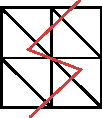
\includegraphics[height=3.5cm]{images/cutting-mig2015/remeshing_1.pdf}
\caption{\label{fig:remeshing1}}
\end{subfigure}
\hfill
\begin{subfigure}[c]{0.3\linewidth}
\centering

\includegraphics[height=3.5cm]{images/cutting-mig2015/remeshing_2.pdf}
\caption{\label{fig:remeshing2}}
\end{subfigure}
\hfill
\begin{subfigure}[c]{0.3\linewidth}
\centering
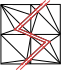
\includegraphics[height=3.5cm]{images/cutting-mig2015/remeshing_3.pdf}
\caption{\label{fig:remeshing3}}
\end{subfigure}
\caption[Frame-based cutting: Remeshing algorithm]{\label{fig:remeshing} Illustration of our remeshing algorithm. (a) For remeshing, we start from an input mesh and a polyline that represents the cut. (b) First we re-mesh along the polyline so that the mesh is conform with the cut. (c) Then we split the mesh vertices along the polyline.}
\end{figure}

\begin{figure}[p]
\centering
\begin{subfigure}[c]{0.3\linewidth}
\centering

\includegraphics[height=3cm]{images/cutting-mig2015/basic_mesh.pdf}
\caption{\label{fig:basicMesh}}
\end{subfigure}
\hfill
\begin{subfigure}[c]{0.3\linewidth}
\centering

\includegraphics[height=3cm]{images/cutting-mig2015/edge_split.pdf}
\caption{\label{fig:edgeSplitting}}
\end{subfigure}
\hfill
\begin{subfigure}[c]{0.3\linewidth}
\centering
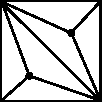
\includegraphics[height=3cm]{images/cutting-mig2015/vertex_insertion.pdf}
\caption{\label{fig:vertexInsertion}}
\end{subfigure}
\caption[Frame-based cutting: Edge splitting and vertex insertion]{\label{fig:operations} Illustrations for edge splitting and vertex insertions. (a) The input mesh. (b) After edge splitting. (c) After vertex insertions.}
\end{figure}

\begin{figure}[p]
\centering
\begin{subfigure}[c]{0.3\linewidth}
\centering

\includegraphics[height=3cm]{images/cutting-mig2015/vertex_splitting_1.pdf}
\caption{\label{fig:vertexSplitting1}}
\end{subfigure}
\begin{subfigure}[c]{0.3\linewidth}
\centering

\includegraphics[height=3cm]{images/cutting-mig2015/vertex_splitting_2.pdf}
\caption{\label{fig:vertexSplitting2}}
\end{subfigure}
\begin{subfigure}[c]{0.3\linewidth}
\centering

\includegraphics[height=3cm]{images/cutting-mig2015/vertex_splitting_3.pdf}
\caption{\label{fig:vertexSplitting3}}
\end{subfigure}
\caption[Frame-based cutting: Vertex splitting]{\label{fig:vertexSplitting} Illustrations for the vertex splitting operation. (a) A mesh which is conform with the polyline (in red). (b) We start by assigning each triangle around the vertex to split to one side of the polyline. (c) We duplicate the vertex and modify each of the triangles accordingly to its side.}
\end{figure}

\clearpage 

%%%%%%%%%%%%%%%%%%%%%%%%%%%%%%%%%%%%%%%%%%%%%%%%%%%%%%%%%%%%%%%%
%                      DISCUSSION 
%%%%%%%%%%%%%%%%%%%%%%%%%%%%%%%%%%%%%%%%%%%%%%%%%%%%%%%%%%%%%%%%
\section{Conclusion} \label{sec:cutting_conclusion}

In this chapter, we presented a novel method to simulate highly detailed cuts with a sparse set of control nodes which allows interactive frame rates. This approach can be seen as a reduced simulation that handles topological changes without requiring expensive precomputations. Of course, our work is not without limitations and brings interesting directions for future work.

Firstly, as very few frames are used, one cut may generate large changes in the weight distribution and produce popping artifacts that cannot be avoided using our interpolation strategy. This is particularly noticeable when simulating soft materials and can be seen in some of the examples of our accompanying video. Strategies proposed by~\cite{Narain2013} and~\cite{Tournier2014} in the context of adaptive simulations could be used to limit this problem. 

Secondly, for large deformations, the surface can look bumpy. There are several reasons for this problem. Linear blend skinning, used to approximate the displacement field, produces well known artifacts that could be solved using a better skinning approach such as dual quaternion skinning. Also, the shape functions derivatives are discontinuous and this is particularly noticeable during high deformations. One could easily change the shape functions and still use the non-manifold grid to depict the topology.

Thirdly, our implementation is far from being optimal. Currently the non-manifold grid and the shape functions are re-computed from scratch at each cut. We could enjoy a dynamic acceleration structure to incrementally update our non-manifold grid. Shape functions could also be incrementally updated. Finally there are several parts of our method that could enjoy parallelization such as samples interpolation.

Finally, we would like to extend our work to 3D. The implementation of our current non-manifold grid would require a tetrahedron representation of the object. We would like to investigate the method of~\cite{Remillard2013} to build this structure only from the object surface. We think that the frame-based framework can be used to produce interactive detailed fracture simulation. The main challenge is to accurately compute stress tensors which are then used to determine fracture direction. Instead of using a dense sampling of frames and integration points to compute the stress tensors, we would like to combine a low resolution stress tensor measurement with procedural detail generation as in the work of~\cite{Chen2014} and~\cite{Lejemble2015}. Finally, we would like to investigate advanced sampling strategies in order to automatically determine how many frames are required for a given region. This would involve the material property, the size and the shape of the region that needs to be sampled.



\backmatter

\printbibliography

\newpage

\listoffigures

\newpage

\listofalgorithms

\newpage

\listoftables

\end{document}
